\documentclass[12pt,a4paper]{amsart}
\usepackage[slovene]{babel}
%\usepackage[cp1250]{inputenc}
%\usepackage[T1]{fontenc}
\usepackage[utf8]{inputenc}
\usepackage{amsmath,amssymb,amsfonts}
\usepackage{url}
\usepackage[shortlabels]{enumitem}
 \usepackage{graphicx}
\usepackage[rightcaption]{sidecap}
\usepackage[export]{adjustbox}
\usepackage{subcaption}
\usepackage{float}
%\usepackage[normalem]{ulem}
\usepackage[dvipsnames,usenames]{color}
\textwidth 15cm
\textheight 24cm
\oddsidemargin.5cm
\evensidemargin.5cm
\topmargin-5mm
\addtolength{\footskip}{10pt}
\pagestyle{plain}

\overfullrule=15pt % oznaci predogo vrstico

\theoremstyle{definition}
\newtheorem{definicija}{Definicija}[section]
\newtheorem{primer}[definicija]{Primer}
\newtheorem{opomba}[definicija]{Opomba}


\theoremstyle{plain}
\newtheorem{lema}[definicija]{Lema}
\newtheorem{izrek}[definicija]{Izrek}
\newtheorem{trditev}[definicija]{Trditev}
\newtheorem{posledica}[definicija]{Posledica}

\newcommand{\Co}{\operatorname{Co}} %konveksna ogrinjača

\newcommand{\LH}{\mathcal{L}}
\newcommand{\R}{\mathbb R}
\newcommand{\N}{\mathbb N}
\newcommand{\Z}{\mathbb Z}
\newcommand{\C}{\mathbb C}
\newcommand{\Q}{\mathbb Q}

\newcommand{\abs}[1]{ \left\lvert#1\right\rvert} 
\newcommand{\norm}[1]{\left\lVert#1\right\rVert}
% vstavi svoje definicije ...

% ukaz za slovarsko geslo
\newlength{\odstavek}
\setlength{\odstavek}{\parindent}
\newcommand{\geslo}[2]{\noindent\textbf{#1}\hspace*{3mm}\hangindent=\parindent\hangafter=1 #2}


%\renewcommand\thesubfigure{\arabic{subfigure}}

\begin{document}


\thispagestyle{empty}
\noindent{\large
UNIVERZA V LJUBLJANI\\[1mm]
FAKULTETA ZA MATEMATIKO IN FIZIKO\\[5mm]
%\textcolor{Red}
{Finančna matematika} -- 1.~stopnja}
\vfill

\begin{center}{\large
Mirjam Pergar\\[2mm]
{\bf Računanje izotropnih vektorjev}\\[10mm]
Delo diplomskega seminarja\\[1cm]
Mentor: prof. dr. Bor Plestenjak}
\end{center}
\vfill

\noindent{\large
Ljubljana, 2017} %letnica diplome
\pagebreak

\thispagestyle{empty}
\tableofcontents
\pagebreak

\thispagestyle{empty}
\begin{center}
{\bf Računanje izotropnih vektorjev}\\[3mm]
{\sc Povzetek}
\end{center}
Delo diplomskega seminarja se ukvarja z izračunom izotropnih vektorjev $b\in\R^{n} (\C^{n})$, ki so rešitev enačbe $b^\ast Ab=0,$ za dano matriko $A\in\R^{n\times n} (\C^{n\times n}), det(A)\ne 0$.
Pomemben pojem pri iskanju teh vektorjev je numerični zaklad, definiran kot $W(A)=\{x^\ast Ax: x \in \C^n,\quad x^\ast x=1\}.$ Predstavljene in dokazane so njegove uporabne lastnosti, kot je npr. konveksnost.
%Na kratko opišemo s katerimi problemi je računanje teh vektorjev povezano.
Računanje izotropnih vektorjev ločimo na 2 dela, in sicer, ko je $A$ realna in ko je kompleksna matrika.
Ko imamo realno matriko, nas v resnici zanima problem $b\ast Hb=0$, za hermitsko matriko $H=(A+A\ast)/2$. 
Pokažemo kako izračunamo 2 izotropna vektorja, če je $A$ nedefinitna, in še več, če ima $H$ vsaj 3 različne lastne vrednosti,ki ne smejo biti istega predznaka, pokažemo, da obstaja neskončno izotropnih vektorjev.
Ko imamo kompleksno matriko, je problem težji in postopkov, kako pridemo do rešitve, več. Predstavimo 3 teoretične postopke Meuranta, Cardna in Chorianopoulos, Psarrakos, Uhliga.
%Za vsak postopek predstavimo potrebne izreke in dodatne konstrukcije, ki se uporabijo, in podrobno opišemo vsak korak v algoritmu.
Meurantov algoritem najprej uporabi lastne vrednosti in vektorje hermitske matrike $K=(A-A\ast)/2\imath$, če to ne deluje uporabi hermitsko matriko $H$, če pa še to ne deluje pa uporabi kombinacijo lastnih vektorjev od $K$ in $H$.
Po tem postopku tudi sprogramiramo kodo v Matlabu.
%V poglavju Numerična analiza najprej opišemo naš algoritem, ki smo ga povzeli po članku Meuranta, in razložimo zakaj se v nekaterih korakih naš algoritem razlikuje od algoritma iz članka.
Nadalje naš algoritem primerjamo z drugima algoritmoma na vseh možnih primerih in ugotovimo \vdots
%Poleg vsakega primera je tudi slika numeričnega zaklada z dodano grafično predstavitvijo iskanja rešitve.
%Na koncu še opišemo naša opazovanja in zaključke.

\vfill
\begin{center}
{\bf The computation of isotropic vectors}\\[3mm]
{\sc Abstract}
\end{center}
The graduation thesis deals with the computation of isotropic vectors $b\in\R^{n} (\C^{n})$, that are solutions of the equation $b^\ast Ab=0,$ for a given matrix $A\in\R^{n\times n} (\C^{n\times n}), det(A)\ne 0$.
An important concept when searching for these vectors is the field of values (or numerical range), defined as $W(A)=\{x^\ast Ax: x \in \C^n,\quad x^\ast x=1\}.$ Some of its useful properties are presented and proved, such as convexity.
%We briefly describe with which problems, the computation of these vectors, are related.
We divide the computation of isotropic vectors into 2 parts, that is when $A$ is a real or a complex matrix.
When we have a real matrix, we are in fact interested in problem $b\ast Hb=0$, for a hermitian matrix $H=(A+A\ast)/2$. 
We show how to compute 2 isotropic vectors, if $A$ is non-definitive, and furthermore, if $H$ has at least 3 distinct eigenvalues of different signs, there exists an infinite number of isotropic vectors.
When we are dealing with a complex matrix the problem is more difficult and more methods of how to find a solution exist. We present 3 theoretical procedures by Meurant, Carden and Chorianopoulos, Psarrakos, Uhlig.
%For every procedure we show needed theorems and extra constructions, that are used, and we describe each step of the algorithm in detail.
Meurant's algorithm first uses eigenvalues and eigenvectors of the hermitian matrix $K=(A-A\ast)/2\imath$, if this does not work it uses hermitian matrix $H$, and if this also does not work it uses a combination of eigenvectors from $K$ and $H$.
We write a code in Matlab after this algorithm.
%In the chapter Numerical analysis we firstly describe our algorithm, which was based of Meurant's paper, and we explain why in some steps in differs from the algorithm in the paper.
Further, we compare our algorithm with the algorithms from the other two papers on every possible example \vdots
%Next to each example we include a picture of the field of values with added graphical illustrations of how we find a solution.
%Lastly we show our observations and conclusions.


\vfill\noindent
{\bf Math. Subj. Class. (2010):15A60, 47A12}   \\[1mm]
{\bf Ključne besede: izotropni vektor, numerični zaklad}   \\[1mm]
{\bf Keywords: isotropic vector, field of values, numerical range}
\pagebreak

%1. poglavje

\section{Uvod}
V uvodnem poglavju bomo predstavili naš problem iskanja izotropnih vektorjev ter vse pojme, ki nam bodo v nadaljnem pomagali pri računanju, kot je numerični zaklad. 
V ostalih poglavjih bomo problem razdelili na realne in kompleksne matrike, ter pojasnili kako izračunamo izotropne vektorje v vsakem primeru.
Na koncu bomo en algoritem implementirali v Matlabu in ga primerjali s še dvema algoritmoma.\\
Sedaj pa opišimo glavni problem tega dela.
\subsection{Problem}

Naj bo $A\in\R^{n\times n} (\C^{n\times n}), det(A)\ne 0$. Iščemo enotski vektor $b\in\R^{n} (\C^{n})$, da je
\begin{equation}\label{eq:zac}
b^\ast Ab=0,
\end{equation}
pravimo mu \emph{izotropni vektor}. \\
%V tem problemu, je neničeln vektor skaliran in rotiran v ortogonalni smeri. %\cite{lipkin}
Bolj splošen je problem \emph{inverznega numeričnega zaklada}, kjer iščemo enotski vektor $b$, za katerega velja:
\begin{equation}\label{eq:splosno}
b^\ast Ab=\mu,
\end{equation}
kjer je $\mu$ dano kompleksno število.\\
Očitno je, da je problem \eqref{eq:splosno} možno prevesti na problem \eqref{eq:zac} za drugo matriko, saj je \eqref{eq:splosno} ekvivalentno
$$b^\ast (A-\mu I)b=0.$$
Zato bomo od sedaj naprej vse vrednosti $\mu$ enačili z $0$.\\
Če je $\mu$ lastna vrednost matrike $A$, torej velja $Av=\mu v$, kjer je $v$ lastni vektor, ki pripada $\mu$, potem je rešitev problema inverznega numeričnega zaklada vektor $v$. 
Če pa $\mu$ ni lastna vrednost matrike $A$, je $A-\mu I$ nesingularna in moramo izotropni vektor izračunati.
Tudi če matrika $A$ ni realna imamo opravka s kompleksno matriko, ko je $\mu$ kompleksno število. 
\begin{izrek}
Naj imata $A$ in $b$ realne ali kompleksne elemente. Potem veljajo enakosti:
$$b^\ast Ab=0\Leftrightarrow b^\ast (A+A^\ast)b=0 \ \textrm{in}\  b^\ast(A-A^\ast)b=0.$$
\end{izrek}
\begin{proof}
($\Rightarrow$) Če velja $b^\ast Ab=0$, je tudi $(b^\ast Ab)^\ast=b^\ast A^\ast b=0$. Če preoblikujemo prvo enačbo na desni v $b^\ast Ab +b^\ast A^\ast b$ dobimo 0. Drugo enačbo dokažemo na podoben način.\\
($\Leftarrow$) S seštevkom enačb na desni dobimo enačbo na levi:
\begin{align*}
 b^\ast (A+A^\ast)b+b^\ast(A-A^\ast)b=0,\\
b^\ast (A+A^\ast+A-A^\ast)b=0,\\
b^\ast (2A)b=0,\\
b^\ast Ab=0.
\end{align*}
\end{proof}

Če velja le $b^\ast (A+A^\ast)b=0$, ugotovimo da je $\Re(b^\ast Ab)=0$. Podobno, če velja samo $b^\ast(A-A^\ast)b=0$, potem je $\Im(b^\ast Ab)=0$. Ta dejstva bomo uporabili pri računanju rešitev za kompleksne matrike. 
Ko sta $b$ in $A$ realna, je problem mnogo enostavnejši, saj moramo upoštevati le simetričen del matrike $A$.\\
Hermitski in poševno-hermitski del matrike $A$ bomo označili s $$H=\frac{A+A^\ast}{2}\quad \text{in} \quad K=\frac{A-A^\ast}{2\imath}.$$

\subsection{Numerični zaklad}
%NUMERIČNI ZAKLAD
\begin{definicija}
\emph{Numerični zaklad} matrike $A \in \C^{n\times n}$ je pod\-mno\-ži\-ca kompleksne ravnine, definirana kot
$$W(A)=\{x^\ast Ax: x \in \C^n,\quad x^\ast x=1\}.$$
\end{definicija}
Očitno je numerični zaklad $W(A)$ množica vseh Rayleighovih kvocientov matrike $A$. Podobno kot spekter (množica vseh lastnih vrednosti matrike) je numerični zaklad množica iz katere lahko razberemo informacije o matriki in pogosto da več informacij kot spekter sam.
%Numerični zaklad vsebuje bistvene informacije o matriki $A$ kot transformaciji, zlasti o lastnih vrednostih in lastnih prostorih (eigenspace) matrike $A$.
Lastne vrednosti hermitskih in normalnih matrik imajo uporabne lastnosti, s katerimi si pomagamo pri izračunu numeričnega zaklada.
Če vzamemo hermitski del matrike se numerični zaklad preslika na realno os in ostane le daljica, kar je podobno kot če bi vzeli realni del kompleksnega števila. Poleg tega ima ta daljica za robova najmanjšo in največjo lastno vrednost matrike.
To prikazuje Slika \ref{fig:zaklad}. (\cite{zaloga})\\
\begin{figure} [h]
\begin{tabular}{lll}
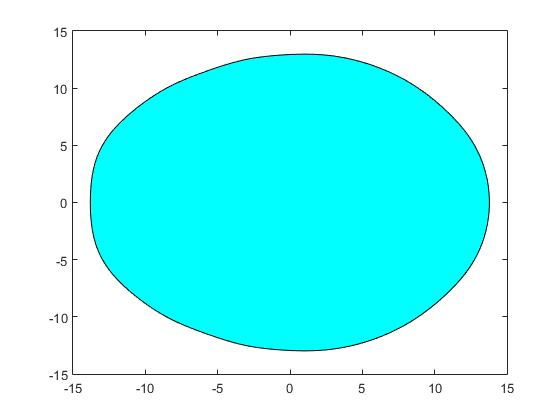
\includegraphics[width=.225\textwidth]{real.jpg}
&
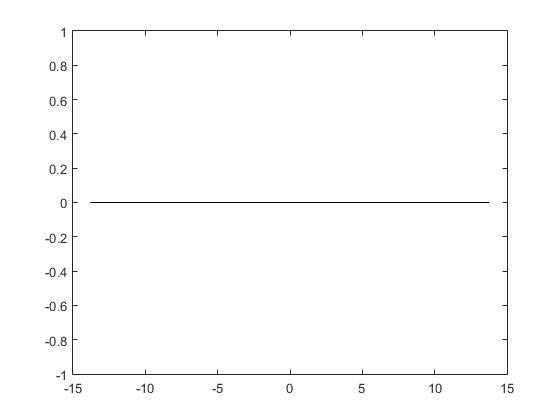
\includegraphics[width=.225\textwidth]{hermit.jpg}
&
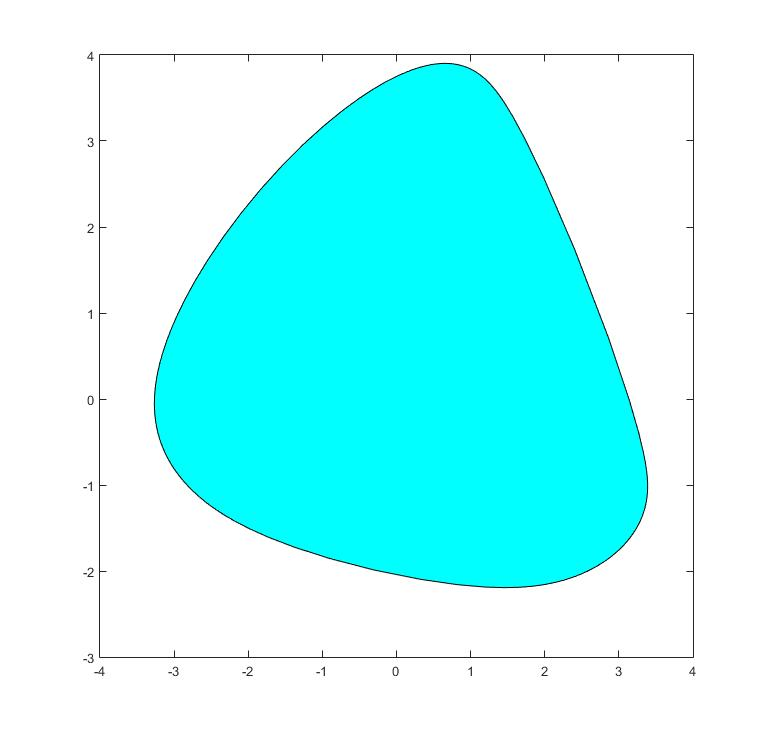
\includegraphics[width=.225\textwidth]{kompleks.jpg}
\end{tabular}
\caption{Numerični zaklad realne, hermitske in kompleksne matrike, narisan z algoritmom opisanem v \cite{zaloga}, ki je dostopen v \cite{nr}.}
\label{fig:zaklad}
\end{figure}


Če hočemo, da ima \eqref{eq:zac} vsaj eno rešitev, mora biti izhodišče vsebovano v $W(A)$. \\

Nekatere lastnosti numeričnega zaklada (\cite{num}, \cite{zaloga}):
\begin{enumerate}{(i)}
\item $W(A)$ je konveksna in kompaktna podmnožica $\C$.
\item $\sigma(A)\subseteq W(A)$, kjer $\sigma(A)$ označuje spekter.
\item Za vsako unitarno matriko $U$ je $W(U^\ast AU)=W(A).$
\item Seštevanje s skalarjem: $W(A+zI)=W(A)+z$ za $\forall z \in \C$.
\item Množenje s skalarjem: $W(zA)=zW(A)$ za $\forall z \in \C$.
\item Subaditivnost: Za $\forall A, B \in \C^{n\times n}$ velja $W(A+B) \subseteq W(A) +W(B).$
\item Projekcija: $W(H)= \Re( W(A))$, za $\forall A\in \C^{n\times n}$, kjer s $H$ označimo hermitsko matriko.
%\item Rob zaloge vrednosti $W(A), \partial W(A)$, je kosoma algebrska krivulja, in vsaka točka v kateri $\partial W(A)$ ni diferenciabilna je lastna vrednost matrike $A$.
\item Če je $A$ normalna, potem $W(A)=\Co(\sigma(A))$, kjer s $\Co$ označimo zaprto konveksno ogrinjačo množice.
\item $W(A)$ je daljica na realni osi, če in samo če je $A$ hermitska.
\end{enumerate}
\begin{proof}
\begin{enumerate}[(i)]
\item
\begin{itemize}
\item Konveksnost: bomo pokazali v naslednjem poglavju.
\item Kompaktnost: Množica $W(A)$ je zaloga vrednosti zvezne funkcije $x \rightarrow x^\ast Ax$ na definicijskem območju $\{x:x\in \C^n , x^\ast x=1\}$ (površina Euklidske enotske krogle), ki je kompaktna množica. Ker je $W(A)$ slika kompaktne množice, pod zvezno funkcijo, sledi da je $W(A)$ kompaktna.
\end{itemize}
\item Predpostavimo, da imamo $\lambda \in \sigma(A)$. Potem obstaja neničeln vektor $x\in \C ^n$ (za katerga lahko predpostavimo, da je enotski), za katerega velja $Ax=\lambda x$ in zato je
$$\lambda = \lambda x^\ast x=x^\ast (\lambda x) = x^\ast Ax \in W(A)$$.
\item Zaradi unitarne transformacije postane površina enotske Evklidske krogle invariantna in so kompleksna števila, ki sestavljajo množici $W(U^\ast AU)$ in $W(A)$ enaka. 
% Ker unitarna transformacija naredi površino Euklidske enotske krogle invariantno, so kompleksna števila, ki sestavljajo množici $W(U^\ast AU)$ in $W(A)$ enaka. 
Če je $x\in \C^n$ in $x^\ast x=1$ imamo $$x^\ast (U^\ast AU)x=y^\ast Ay \in W(A),$$ kjer je $y = Ux$, torej $$y^\ast y=x^\ast U^\ast Ux=x^\ast x=1.$$ Torej je $W(U^\ast AU)\subseteq W(A)$. 

\item Imamo 
\begin{align*}
W(A +zI)&=\{x^\ast (A+zI)x: x^\ast x=1\}\\
& = \{x^\ast Ax + zx^\ast x: x^\ast x =1\}\\
 &= \{x^\ast Ax + z: x^\ast x=1\} \\
&= \{x^\ast Ax: x^\ast x=1\} +z \\
&= W(A) +z.
\end{align*}
\item Imamo 
\begin{align*}
W(zA) &= \{x^\ast (zA)x: x^\ast x=1\}\\
& = \{zx^\ast Ax:x^\ast x =1\}\\
&= z\{x^\ast Ax:x^\ast x=1\}\\
& = zW(A).
\end{align*}

\item Imamo
\begin{align*}
W(A+B)&=\{x^\ast(A+B)x: x\in \C^n, x^\ast x=1\}\\
& = \{x^\ast Ax +x^\ast Bx: x\in \C^n, x^\ast x=1\}\\
& \subseteq \{x^\ast Ax: x\in \C^n, x^\ast x=1\}+\{yx^\ast By: y\in \C^n, y^\ast y=1\}\\
& =W(A) + W(B).
\end{align*}
\item Računamo
\begin{align*}
x^\ast Hx &= x^\ast \frac{1}{2}(A+A^\ast)x \\
 &=\frac{1}{2} (x^\ast Ax +x^\ast A^\ast x) \\
 &=\frac{1}{2}(x^\ast Ax +(x^\ast Ax)^\ast) \\
 &= \frac{1}{2}(x^\ast Ax +\overline{x^\ast Ax}) \\
 &= \Re (x^\ast Ax).
\end{align*}

\item Če je A normalna, potem je $A=U^\ast \Lambda U$, kjer je $\Lambda = \text{diag}\{\lambda_1, \dots, \lambda_n\}$ diagonalna in $U$ unitarna. 
Po lastnosti (3) je $W(A)=W(\Lambda)$ in ker $$x^\ast \Lambda x = \sum_{i=1}^{n} \bar{x}_i x_i\lambda_i = \sum_{i=1}^{n} |x_i|^2 \lambda_i$$ 
je $W(\Lambda)$ množica vseh konveksnih kombinacij diagonalnih elementov $\Lambda$ ($x^\ast x=1$ implicira $ \sum_{i} |x_i|^2 =1$ in $|x_i|^2 \geq 0$). 
Ker so diagonalni elementi $\Lambda$ lastne vrednosti $A$, to pomeni da je $W(A) =\Co(\sigma(A))$

\item Ker je hermitska matrika tudi normalna velja $$W(H) = \Co(\sigma(H)),$$ zaradi lastnosti (3). 
Vemo, da se numerični zaklad hermitske matrike projecira na realno os ter da je $\sigma(H)$ množica vseh realnih lastnih vrednosti matrike $H$. 
Konveksna ogrinjača $\sigma(H)$ je množica vseh daljic med lastnimi vrednostmi matrike $H$ in ker bo numerični zaklad samo na realni osi, je to daljica med najmanjšo in največjo realno lastno vrednostjo $H$.
\end{enumerate}
\end{proof}
\subsubsection{Konveksnost}
V tem poglavju bomo dokazali, da je numerični zaklad konveksen, kar je znano tudi kot Toeplitz-Hausdorfferjev izrek. 
Načinov kako dokazati konveksnost je več, npr. \cite{num}, vendar bomo mi izrek dokazali tako kot je dokazan v \cite{zaloga}, za to pa potrebujemo dodatno lemo. 
\begin{lema}
Naj bo $H\in \C^{n\times n}$ hermitska matrika in $\mu \in W(H)$. Potem je množica $\LH _{H}(\mu)=\{x\in \C^n:\quad x^\ast x=1,\quad x^\ast Hx=\mu\}$ povezana s potmi (t.j. obstaja pot med poljubnima dvema točkama iz te množice)% oz. poljubni dve točki iz te množice lahko povežemo z zvezno krivulju, ki je v celoti vsebovana v množici)
\end{lema}

\begin{proof}
Zaradi lastnosti (3) in (4) lahko brez škode za splošnost predpostavimo, da je $\mu=0$ in $H=\text{diag}\{d_1,d_2,\dots,d_n\}$ realna diagonalna matrika.
Potem je 
$$W(H)=\Big\{ \sum_{j=1}^{n} d_j|x_j|^2:\quad x_1,x_2,\dots,x_n \in \C,\quad \sum_{j=1}^{n} |x_j|^2=1\Big \}$$
Naj bo sedaj $x=(x_j), y=(y_j)\in \LH_{H}(0)$ t.j. $x,y$ sta enotska vektorja za katera velja 
$$\sum_{j=1}^{n} d_j|x_j|^2=\sum_{j=1}^{n} d_j|y_j|^2=0.$$
 Pokazati želimo, da v $\LH_{H}(0)$ obstaja zvezna pot, ki povezuje $x$ in $y$. Ker je vsak vektor 
$$\Big[r_1 e^{i\theta_1}\quad  r_2 e^{i\theta_2}\quad  \dots\quad r_n e^{i\theta_n}\Big]^T \in \LH_{H}(0)$$  
$(r_j \geq 0, \theta_j\in [o, 2\pi); j=1,2,\dots,n)$ povezan z realnim vektorjem 
$$[r_1 \quad r_2 \quad \dots \quad r_n]^T \in \LH_{H}(0)$$
 z zvezno krivuljo
$$\Big[r_1 e^{i\theta_1(1-t)}\quad  r_2 e^{i\theta_2(1-t)}\quad  \dots\quad  r_n e^{i\theta_n(1-t)}\Big]^T; \quad t\in[0,1],$$
ki je v $\LH_{H}(0)$, sleda, da sta $x$ in $y$ realna in nenegativna. Potem zvezna krivulja
$$u(t)=(u_j(t))=\Big(\sqrt{(1-t)x^2_j -ty^2_j}\Big) \in \LH_{H}(0)\cap \R^n ; \quad t\in [0,1]$$
zadošča pogojema $u (0)=x$ in $u (1) =y$, s čimer je lema dokazana.
\end{proof}

Seveda, zgornja lema drži za vsako skalarno množenje hermitske matrike. 
Še več, za realno diagonalno matriko $H=\text{diag}\{d_1,d_2,\dots,d_n\}$, $d_1\geq d_2\geq \dots \geq d_n$, vrednost $\sum_{j=1}^{n} d_j|x_j|^2$ 
(kjer je $x_1,x_2,\dots, x_n \in \C,\quad \sum_{j=1}^{n}|x_j|^2 =1$) doseže maksimum $d_1$, pri $|x_1|=1$ in $x_2=x_3=\dots=x_n=0$ in doseže minimum $d_n$, pri $|x_n|=1$ in $x_1=x_2=\dots=x_{n-1}=0$. Velja naslednja posledica.

\begin{posledica}
Naj bo $H\in \C^{n\times n}$ hermitska matrika in $\mu$ njena najmanjša ali največja lastna vrednost. Potem množica $\LH_{H}(\mu)=\{x\in \C^n:\quad x^\ast x=1,\quad x^\ast Hx=\mu \}$ vsebuje vse enotske lastne vektorje matrike $H$, ki pripadajo $\mu$.
\end{posledica}

\begin{izrek}[\emph{Toeplitz-Hausdorfferjev izrek}]
Za $\forall A\in \C^{n\times n}$ je $W(A)$ konveksna.
\end{izrek}

\begin{proof}
Dokazati moramo, da če vzamemo poljubni točki $\mu, \nu \in W(A)$,  mora daljica s krajiščema $\mu$ in $\nu$ ležati v $W(A)$. Zaradi lastnosti (4) lahko brez škode za splošnost predpostavimo, da sta $\mu=0$ in $\nu=1$. Naj bosta $x,y\in \C^n$ taka enotska vektorja, da velja $x^\ast Ax=0$ in $y^\ast Ay=1$. 
Naj bo $H$ hermitski del matrike $A$ in $\tilde{K}$ poševno-hermitski del matrike $A$, kot smo jih definirali v prejšnjem podpoglavju. Množica $\LH_{\tilde{K}}(0) =\{x\in \C^n:\quad x^\ast x=1,\quad x^\ast Kx=0\}$ je zaradi prejšnje leme povezana s potmi. Ker sta $x,y\in \LH_{K}}(0)$, obstaja taka zvezna vektorska funkcija $z(t): [0,1] \rightarrow \LH_{K}(0)$, da sta $z(0)=x$ in $z(1)=y$.  Sledi, da je funkcija 
\begin{align*}
z(t)^\ast A z(t) &= z(t)^\ast Hz(t) +z(t)^\ast K z(t) \\
 &= z(t)^\ast Hz(t)
\end{align*}
realna in zvezna glede na spremenljivko $t$ in zadošča pogojema $$z(0)^\ast Az(0)=x^\ast Ax=0$$ in $$z(1)^\ast Az(1)=y^\ast Ay=1.$$ Sledi, da je daljica s krajiščema $0$ in $1$ vsebovana v $W(A)$.
\end{proof}

\subsection{Uporaba}
Zanimanje za izračun izotropnih vektorjev je povezano s pre\-u\-če\-va\-njem delne stagnacije GMRES algoritma za reševanje linearnih sistemov z realnimi matrikami. Numerični zaklad se uporablja za preučevanje konvergence nekaterih iterativnih metod za reševanje linearnih sistemov in ima mnogo aplikacij v numerični analizi, diferencialnih enačbah, teoriji sistemov itd.
%%%%%%%%%%%%%%%%%%%%%%%%%%%%%%%%%%%%%%%%%%%%%%%%%%%%%%%%%%%%%%%%%%%%%%%%%%%%%%%%%%%%%%%%%%%%%%%%%%%%%%%%%%%%%%%%%%%%%%%%%%%%%%%%%%%%%%%%%%%%%%%%%%%%%%%%%%%%%%%%%%%%%%%%%%%%%%%%%%%%%%
%2. poglavje

\section{Realne matrike}\label{Realne matrike}
V tem razdelku bomo opisali kako izračunamo željeno število izotropnih vektorjev za realno matriko, kot je predstavjeno v članku \cite{meurant}. To storimo z uporabo lastnih vektorjev matrike $$H=\frac{A+A^\ast}{2}.$$\\
Ko je $A$ realna matrika, nas zanima, kako izračunati rešitev naslednje enačbe:
\begin{equation}\label{eq:realna}
b^\ast Hb=0,
\end{equation}
kjer je $H$ realna in simetrična matrika (t.j. $H=H^T$).
\begin{lema} \cite{lipkin}
Izotropni vektorji realne matrike A so identični izotropnim vektorjem njenega simetričnega dela.
\end{lema} 
\begin{proof}
To sledi iz $b^T Ab=b^T A_{sim} b +b^T A_{psim} b=b^T A_{sim} b,$ kjer je z $A_{sim}=\frac{A+A^T}{2}$ označen simetrični del matrike $A$ in z $A_{psim}=\frac{A-A^T}{2}$ poševno-simetrični del matrike A.
\end{proof}
Velja enakost:
$$b^T Ab=0 \Leftrightarrow b^T (A+A^T)b=0.$$  
Vemo, da je $W(A)$ simetrična glede na realno os in, da je $0 \in W(A)$, če in samo če $\lambda_n\le0\le\lambda_1$, kjer sta $\lambda_n$ najmanjša in $\lambda_1$ največja lastna vrednost matrike $H$. Naj bosta $x_1$ in $x_n$ realna lastna vektorja, pripadajoča $\lambda_1$ in $\lambda_n$.  Potem sta $x_1^T Ax_1=x_1^T Hx_1=\lambda_1$ in $x_n^T Ax_n=x_n^T Hx_n=\lambda_n$ realni točki na skrajni levi in skrajni desni zaloge vrednosti $W(A)$ na realni osi.\\

Realne rešitve \eqref{eq:realna} izračunamo z uporabo lastnih vektorjev matrike $H$. Predpostavimo, da iščemo vektorje $b$ z normo 1. Matriko $H$ lahko zapišemo kot $$H=X\Lambda X^T,$$ kjer je $\Lambda$ matrika, ki ima na diagonali lastne vrednosti $\lambda_i$, ki so realna števila. $X$ je ortogonalna matrika lastnih vektorjev, tako da $X^T X=I$. Potem uporabimo ta spektralni razcep v \eqref{eq:realna}: $$b^\ast Hb=b^\ast X\Lambda X^T b=0.$$ Označimo s $c=X^Tb$ vektor projekcije $b$ na lastne vektorje matrike $H$. Dobimo naslednji izrek.
\begin{izrek} \label{izrek2}
Naj bo $b$ rešitev problema \eqref{eq:realna}. Potem vektor $c=X^T b$ s komponentami $c_i$ zadošča naslednjima enačbama:
\begin{align}
\sum_{i=1}^{n} \lambda_i \abs{c_i}^2=0 \label{eq:en1},\\
\sum_{i=1}^{n}\abs{c_i}^2=1. \label{eq:en2}
\end{align}
\end{izrek}
\begin{proof}
Enačbo \eqref{eq:en1}  dokažemo tako, da $c=X^Tb$ oz. $c^\ast =b^\ast X$ vstavimo v \eqref{eq:realna} in dobimo $$b^\ast Hb=b^\ast X\Lambda X^T b= c^\ast \Lambda c=0.$$ Ker je $\Lambda$ diagonalna matrika, lahko $c^\ast \Lambda c$ zapišemo kot vsoto komponent $\bar{c_i}\lambda_i c_i=\lambda_i\abs{c_i}^2$, za $i=1,2,...n$.
Za enačbo \eqref{eq:en2} vemo, da je $\norm{b}_2=1$. Če normo zapišemo s $c$, dobimo $$\norm{b}_2=\norm{Xc}_2=\norm{c}_2=1,$$ saj je $X$ ortogonalna matrika.

\end{proof}
%\begin{bmatrix}
%$\lambda_1$ & &\\
% &\ddots& \\
% & &$\lambda_n$
%\end{bmatrix}
\begin{opomba}
Enačbi veljata samo za realna števila. Zaradi  izreka \ref{izrek2} mora biti 0 konveksna kombinacija lastnih vrednosti $\lambda_i$. Kot smo že videli, to pomeni, da če je $A$ definitna matrika (pozitivno ali negativno), potem \eqref{eq:realna}
nima netrivialne rešitve. Drugače je $0 \in W(A)$ in lahko vedno najdemo realno rešitev. V bistvu, kadar je $n>2$, lahko najdemo neskončno izotropnih vektorjev.
\end{opomba}
\subsection{Iskanje izotropnih vektorjev}
Najprej bomo pokazali kako izračunamo izotropne vektorje, če imamo dve lastni vrednosti, kasneje pa če imamo tri lastne vrednosti.\\

Če niso vse lastne vrednosti $H$ enako predznačene, potem mora za najmanjšo lastno vrednost $\lambda_n$ veljati $\lambda_n <0$. 
Naj bo $k<n$ tak, da je $\lambda_k >0$ in naj bo $t$ pozitivno realno število manjše od 1.  Izberemo taka $c_n$ in $c_k$, da velja  $\abs{c_n}^2 =t$, $\abs{c_k}^2=1-t$ in $c_i =0, i\not=n,k$, ker velja enačba \eqref{eq:en2}, $t+ (1-t)=1$. Iz \eqref{eq:en1} mora veljati enačba: $$\lambda_n t +\lambda_k (1-t)=0,$$ katere rešitev je:
\begin{equation}
t_s=\frac{\lambda_k}{\lambda_k -\lambda_n}.
\end{equation}
Ker je $\lambda_n <0$, je imenovalec pozitiven in $t_s$ pozitiven ter $t_s <1$. Absolutna vrednost $c_n$ (oz. $c_k$) je kvadratni koren $t_s$ (oz. $1-t_s$). Ker je $b=Xc$, sta realni rešitvi: $$b_1=\sqrt{t_s}x_n +\sqrt{1-t_s}x_k,\quad b_2=-\sqrt{t_s}x_n+\sqrt{1-t_s}x_k,$$ kjer sta $x_n$ in $x_k$ lastna vektorja, ki pripadata lastnima vrednostima $\lambda_n$ in $\lambda_k$. Druge možnosti za predznak dajo rešitve, ki so v isti smeri kot ti dve. Ker imata izraza v rešitvah enaka imenovalca, lahko rešitvi zapišemo kot: $$b_1=\sqrt{\lambda_k}x_n+\sqrt{\abs{\lambda_n}}x_k, \quad b_2=-\sqrt{\lambda_k}x_n+\sqrt{\abs{\lambda_n}}x_k$$(sledi iz \cite{lipkin}).  Vektor mora biti normiran, zato
%NORMIRANI
 $$b_1=\sqrt{\frac{\lambda_k}{\lambda_k +\abs{\lambda_n}}}x_n + \sqrt{\frac{\abs{\lambda_n}}{\lambda_k +\abs{\lambda_n}}}x_k,\quad b_2=-\sqrt{\frac{\lambda_k}{\lambda_k +\abs{\lambda_n}}}x_n + \sqrt{\frac{\abs{\lambda_n}}{\lambda_k +\abs{\lambda_n}}}x_k.$$ \\%V principu  lahko te $b$-je pomnožimo s $e^{i\theta}$, ampak nam to vrne rešitev v isti smeri. \\
 Konstruirani rešitvi sta neodvisni in še več, ortogonalni, če $\lambda_k =-\lambda_n$. \\
%V bistvu lahko uporabimo vsak par pozitivnih in negativnih lastnih vrednosti. Ta postopek lahko vrne toliko rešitev kot je dvakratno število parov lastnih vrednosti matrike $H$ z nasprotnimi predznaki, če so vse lastne vrednosti različne. Konstruirani rešitvi sta neodvisni in še več, ortogonalni, če $\lambda_k =-\lambda_n$. \\
Predpostavimo, da je $b$ realen.
\begin{posledica}\cite{lipkin}
Dobljena izotropna vektorja sta ortogonalna ($b_1 ^T b_2=0$), če in samo če $\lambda_k=-\lambda_n$.
\end{posledica}
\begin{proof}%gleda wi kot negativno, mi pa mamo abs
$$b_1 ^T b_2=(\sqrt{\lambda_k}x_n+\sqrt{\abs{\lambda_n}}x_k)^T (-\sqrt{\lambda_k}x_1+\sqrt{\abs{\lambda_n}}x_k )= -(\lambda_n +\lambda_k).$$
\end{proof}
Za ta postopek lahko uporabimo vsak par pozitivnih in negativnih lastnih vrednosti, uporaba najmanjše lastne vrednosti $\lambda_n$ torej ni nujna. Tako lahko postopek vrne toliko rešitev kot je dvakratno število parov lastnih vrednosti matrike $H$ z nasprotnimi predznaki, če so vse lastne vrednosti različne.\\
Ko sta $A$ in $b$ realna smo dokazali naslednji izrek:
\begin{izrek}
Če je $A$ realna in nedefinitna (t.j. ni pozitivno in negativno definitna), potem obstajata najmanj dva neodvisna realna izotropna vektorja.
\end{izrek}
Da bi pokazali, da imamo neskončno število realnih rešitev in, da bi jih nekaj izračunali, moramo vzeti vsaj tri različne lastne vrednosti, ki ne smejo biti istega predznaka (ko obstajajo). Predpostavimo, da imamo $\lambda_1 <0<\lambda_2<\lambda_3$ in naj bo $t_1=\abs{c_1}^2$, $t_2=\abs{c_2}^2$. Veljati mora enačba \eqref{eq:en2}
\begin{equation}\label{trije}
\lambda_1 t_1 +\lambda_2 t_2 +\lambda_3 (1- t_1 -t_2)=(\lambda_1 -\lambda_3)t_1 +(\lambda_2 -\lambda_3)t_2 +\lambda_3=0
\end{equation}
s pogoji: $t_i \ge 0, i=1,2$ in $t_1 +t_2\le1$. Torej velja zveza $$t_2=\frac{\lambda_3}{\lambda_3 - \lambda_2} -\frac{\lambda_3 -\lambda_1}{\lambda_3 -\lambda_2}t_1.$$
S tem je definirana premica v $(t_1,t_2)$ ravnini in preveriti moramo, če ta premica seka trikotnik, definiran s pogoji za $t_1,t_2$. Premica seka $t_1$-os pri $\lambda_3 /(\lambda_3 -\lambda_1)$, kar je več kot 1, saj je $\lambda_1 <0$, $t_2$-os pa pri $\lambda_3 /(\lambda_3 - \lambda_2)$, kar je tudi več kot 1. Ta premica ima negativen naklon. Vse dopustne vrednosti za $t_1$ in $t_2$ so dane z daljico v trikotniku. Zato obstaja neskončno število možnih pozitivnih parov $(t_1,t_2)$.(\cite{meurant})
%%%%%%%%%%%%%%%%%%%%%%%%%%%%%%%%%%%%%%%%%%%%%%%%%%%%%%%%%%%%%%%%%%%%%%%%%%%%%%%%%%%%%%%%%%%%%%%%%
%%%%%%%%%%%%%%%%%%%PRIIIIIIIIIIIIIMEEEEEEEEEEEEEEEEEEEEEEEEEEEEEEEEEEERRRRRRRRRRRRRRRRRRRRRR%%%%%%%%%%%%%%%%%%%%%%
\begin{primer}
Poglejmo si enostaven zgled za matriko $3x3$ z lastnimi vrednostmi $\lambda_1=-1, \lambda_2=1$ in $\lambda_3=2$.
Matrika lastnih vektorjev $X$ je enaka identiteti $I$.\\
Enačba premice je $t_2=2-3t_1$ s pogoji $t_1, t_2 \ge 0$ in $t_1+t_2\le 1$.\\
Dopustne rešitve za $t_1$ in $t_2$ so dane z daljico v trikotniku, %Slika \ref{fig:daljica}.\\
%\begin{figure}
%\centering
%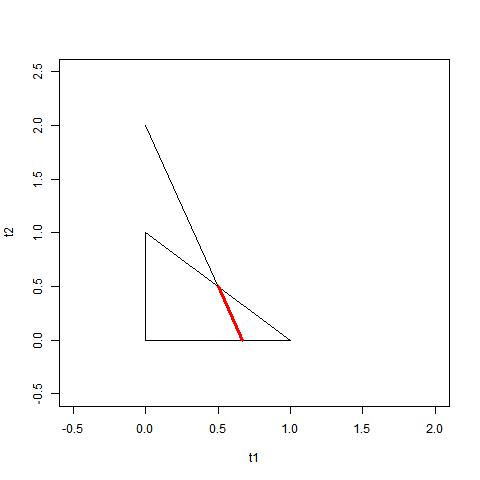
\includegraphics[width=7cm]{graf3.jpg}
%\caption{Dopustne rešitve so na daljici, pobarvani rdeče, v trikotniku omejitev.}
%\label{fig:daljica}
%\end{figure}

Iz daljice lahko izberemo katerikoli par točk $(t_1, t_2)$, npr. $(0.5, 0.5)$. Potem vemo kako izgleda vektor 
$c=\begin{bmatrix}
\sqrt{0.5}\\
\sqrt{0.5}\\
0
\end{bmatrix}$. Iz enačbe $c=X^T b$ dobimo 
$$b=Xc=c =\begin{bmatrix}
\sqrt{0.5}\\
\sqrt{0.5}\\
0
\end{bmatrix}.$$
Seveda je rešitev tudi $b=-c$. Tako lahko izračunamo neskončno izotropnih vektorjev $b$.
\end{primer}
Primer $\lambda_1 <\lambda_2<0<\lambda_3$ je podoben zgornjemu, le da premica seka $t_2$-os pod 1. Potem dobimo rešitve $b$ s kombiniranjem pripadajočih treh lastnih vektorjev. %Ta problem za iskanje koeficientov je v treh dimenzijah in možne rešitve $t$-ja so v eni dimenziji. 
Takšna konstrukcija pripelje do naslednjega izreka:
\begin{izrek}
Če je $n>2$ in je $A$ realna in nedefinitna, potem ima matrika $H$ vsaj tri različne lastne vrednosti z različnimi predznaki. Potem obstaja neskončno število realnih izotropnih vektorjev.
\end{izrek}
%dokaz v citat
Seveda lahko nadaljujemo z večanjem števila lastnih vrednosti. Če uporabimo štiri različne lastne vrednosti z različnimi predznaki, potem moramo na problem gledati v treh dimenzijah. Prostor, kjer je omejitvam zadoščeno, je tetraeder, torej moramo poiskati presek dane ravnine s tem tetraedrom. 
V splošnem, če imamo $k$ različnih lastnih vrednosti z različnimi predznaki, definira naš problem naslednja enačba:
\begin{equation}
\sum_{i=1}^{k-1} (\lambda_i -\lambda_k)t_i +\lambda_k =0, \quad t_i\ge0, i=1, \dots,k-1, \quad \sum_{i=1}^{k-1}t_i \le1.
\end{equation}
Prva enačba opisuje hiperravnino v kateri moramo poiskati  presečišča te hiperravnine z volumnom telesa definiranega s pogoji.
Če je $A$ realna matrika smo končali, saj smo pokazali, da lahko poračunamo toliko realnih rešitev kot hočemo. (\cite{meurant})

%%%%%%%%%%%%%%%%%%%%%%%%%%%%%%%%%%%%%%%%%%%%%%%%%%%%%%%%%%%%%%%%%%%%%%%%%%%%%%%%%%%%%%%%%%%%%%%%%%%%%%%%%%%%%%%%%%%%%%%%%%%%%%%%%%%%%%%%%%%%%%%%%%%%%%%%%%%%%%%
%3. poglavje
\section{Kompleksne matrike}
V tem razdelku si bomo pogledali kako se računa izotropne vektorje, ko je $A$ kompleksna matrika. Predstavljeni bodo trije teoretični postopki iz \cite{meurant},\cite{carden} in \cite{trije}, kako priti do izotropnih vektorjev.
\subsection{Iskanje izotropnih vektorjev}
%MEURANT
\subsubsection{Meurant 1.}
V nekaterih primerih lahko izračunamo rešitve s samo enim ra\-ču\-na\-njem lastnih vrednosti in vektorjev matrike $K$, vendar to ne deluje vedno. Sredstvo, ki lahko pomaga je, da uporabimo lastne vektorje matrike $H$. 
Če ima matrika $A$ kompleksne elemente, nam prejšnja konstrukcija za realne matrike vrne le vektorje za katere je $\Re(b^\ast Ab)=0$. 
Najprej opazimo, da lahko v nekaterih primerih uporabimo podobno konstrukcijo kot v prejšnjem razdelku, ki najde množico rešitev za hermitsko matriko $H$ z ničelnim realnim delom ter pozitivnim in negativnim imaginarnim delom. 
Z uporabo treh lastnih vektorjev $H$, obstaja neskončno rešitev dobljenih na daljici v trikotniku omejitev. 
Ko poljubno točko iz daljice nenehno sprehajamo po tej daljici, se tudi imaginarni del rešitve nenehno spreminja. 
Če sta imaginarna dela, ki ustrezata robnima točkama daljice, različnih predznakov, potem iz izreka o povprečni vrednosti sledi, da obstaja točka na daljici, ki ima ničeln imaginarni del. (\cite{meurant}) \\
%??T%WTFo se lahko izračuna z dihotomijo??. 
\begin{opomba}
To vsebuje samo izračun kvadratne forme $x^\ast Ax$. Ne potrebujemo nobenih izračunov lastnih vrednosti in vektorjev. Vendar, se sprememba predznaka v vrednostih $x^\ast Ax$ ne zgodi za katerkoli tri lastne vrednosti.
\end{opomba}
\subsubsection{Meurant 2.}\label{Meurant 2}
Druga konstrukcija algoritma v \cite{meurant} uporabi lastne vrednosti in lastne vektorje matrike $K=(A-A^\ast)/(2i)$, ki je hermitska. 
S konstrukcijo iz 2. razdelka lahko poiščemo tak vektor $b$, da je $\Im(b^\ast Ab)=0$. 
S kombiniranjem lastnih vektorjev matrike $K$ pripadajočim k pozitivnim in negativnim lastnim vrednostim, lahko (v nekaterih primerih) izračunamo taka vektorja $b_1$ in $b_2$, da $\alpha_1=\Re(b_1^\ast Ab_1)<0$ in $\alpha_2=\Re(b_2^\ast Ab_2)>0$. 
%POMEMBNA LEMA
\begin{lema}\label{komp}
Naj bosta $b_1$ in $b_2$ enotska vektorja z $\Im(b_i^\ast Ab_i)=0$, $i=1,2$, in $\alpha_1=\Re(b_1^\ast Ab_1)<0, \alpha_2=\Re(b_2^\ast Ab_2)>0$. Naj bo 
$$b(t,\theta)=e^{-i\theta}b_1 + tb_2, \quad t,\theta \in \R,$$ 
$$\alpha(\theta)=e^{i\theta}b_1^\ast Ab_2 +e^{-i\theta}b_2^\ast Ab_1.$$
Potem je 
$$b(t,\theta)^\ast Ab(t,\theta)=\alpha_2 t^2 +\alpha(\theta)t+\alpha_1,\quad \alpha(\theta)\in\R,$$ ko 
$$\theta=\text{arg}(b_2^\ast Ab_1 -b_1^T\bar{A}\bar{b_2}).$$ Za 
$$t_1 = \frac{-\alpha(\theta) + \sqrt{\alpha(\theta)^2 - 4\alpha_1 \alpha_2}}{2\alpha_2}$$ imamo 
$$b(t_1, \theta) \not=0,\quad  \frac{b(t_1,\theta)^\ast}{\norm{b(t_1,\theta)}}A\frac{b(t_1,\theta)}{\norm{b(t_1,\theta)}}=0.$$
\end{lema}
Lema \ref{komp} prikazuje kako se izračuna rešitev iz $b_1$ in $b_2$. Če imamo $b_1$ in $b_2$, taka da  $\alpha_1=\Re(b_1^\ast Ab_1)<0$ in $\alpha_2=\Re(b_2^\ast Ab_2)>0$, smo končali.(\cite{meurant})
\begin{proof}
Imamo enotska vektorja $b_1, b_2$ za katera velja $\Im(b_i^\ast Ab_i)=0$, $i=1,2$ in $\alpha_1=\Re(b_1^\ast Ab_1)<0, \alpha_2=\Re(b_2^\ast Ab_2)>0$. Radi bi, da velja
$$\Re(b(t,\theta)^\ast Ab(t,\theta))=0 \quad t,\theta \in \R.$$
\begin{align*}
b(t,\theta)^\ast Ab(t,\theta) &=(e^{-i\theta}b_1 + tb_2)^\ast A (e^{-i\theta}b_1 + tb_2)\\
& = (b_{1}^\ast(\overline{e^{-i\theta}})^T  +b_{2}^\ast t ) A (e^{-i\theta}b_1 + tb_2)\\
& = (b_{1}^\ast(e^{\overline{-i\theta}})^T + b_{2}^\ast t) A (e^{-i\theta}b_1 + tb_2)\\
& = (b_{1}^\ast(e^{i\theta})^T A+ b_{2}^\ast t A) (e^{-i\theta}b_1 + tb_2)\\
& = b_1 ^\ast e^{i\theta} A e^{-i\theta}b_1 + b_1 ^\ast e^{i\theta} A tb_2 + b_2 ^\ast t A e^{-i\theta} b_1 + b_2 ^\ast t Atb_2\\
& = b_1 ^\ast Ab_1 + e^{i\theta} b_1 ^\ast A b_2 t + e^{-i\theta}b_2 ^\ast Ab_1 t + t^2 b_2 ^\ast Ab_2\\
\end{align*}
Če gledamo samo realni del zadnje vrstice dobimo naslednjo kvadratno enačbo:
$$\alpha _1 +  \alpha(\theta)t +  \alpha_2 t^2 =0.$$
Ena rešitev te enačbe je 
$$t_1 = \frac{-\alpha(\theta) + \sqrt{\alpha(\theta)^2 - 4\alpha_1 \alpha_2}}{2\alpha_2}.$$
Preveriti je potrebno le še kdaj bo $$\alpha(\theta)=e^{i\theta}b_1^\ast Ab_2 +e^{-i\theta}b_2^\ast Ab_1 \in \R.$$
To bo držalo, ko bo $$\theta = \text{arg}(b_2^\ast Ab_1 - \overline{b_1^\ast Ab_2}) = \text{arg}(b_2^\ast Ab_1 -b_1^T\bar{A}\bar{b_2}).$$
\end{proof}
\paragraph{Algoritem:}
\begin{enumerate}[1.]
\item S kombiniranjem lastnih vektorjev $K$, pripadajočim pozitivnim in negativinim lastnim vrednostim, izračunamo vektorja $b_1$ in $b_2$, taka da  $\alpha_1=\Re(b_1^\ast Ab_1)<0$ in $\alpha_2=\Re(b_2^\ast Ab_2)>0$. Uporabimo lemo \ref{komp} in končamo.
\item Če ne najdemo $b_1$, $b_2$ potrebna za lemo \ref{komp}, izračunamo še lastne vektorje matrike $H$.  Ponovimo korak 1. za matriko $\imath A$.
\item Če postopek ne deluje niti za $\imath A$, uporabimo kombinacijo lastnih vektorjev $K$ in $H$, kjer z $x$ označimo lastni vektor $K$ in z $y$ lastni vektor $H$.
\item Upoštevamo vektorje $X_\theta =\cos(\theta)x+\sin(\theta)y,$ $0\le\theta\le\pi$. $X_\theta ^\ast AX_\theta$ opiše elipso znotraj numeričnega zaklada.
\item Za dan par $(x,y)$ iščemo presečišča elipse $X_\theta ^\ast AX_\theta$ z realno osjo. Z u\-po\-šte\-va\-njem, da je $A=H+iK$, računamo:
\begin{align*}
X_\theta^\ast AX_\theta &= \cos^2(\theta)(x^\ast Hx + ix^\ast Kx)\\ 
&+ \sin^2(\theta)(y^\ast Hy + iy^\ast Ky)\\ 
&+\sin(\theta)\cos(\theta)(x^\ast Hy +y^\ast Hx +i[x^\ast Ky +y^\ast Kx]).
\end{align*}
Naj bo $\alpha=\Im(x^\ast Hx + ix^\ast Kx), \beta=\Im(y^\ast hy +iy^\ast Ky)$ in $\gamma=\Im(x^\ast Hy +y^\ast Hx +i[x^\ast Ky +y^\ast Kx]).$ Ko izenačimo imaginarni del $X_\theta ^\ast AX\theta$ z 0, dobimo enačbo:
$$\alpha \cos^2(\theta) +\beta \sin^2(\theta) +\gamma \sin(\theta)\cos(\theta)=0.$$
Predpostavimo, da $\cos(\theta) \not =0$ in delimo, dobimo kvadratno enačbo za $t=\tan(\theta),$
$$\beta t^2 +\gamma t +\alpha =0.$$
\item Če ima ta enačba realne rešitve, potem dobimo vrednosti $\theta$, ki nam vrnejo take vektorje $X_\theta$, da $\Im(X_\theta ^\ast AX_\theta)=0$.
\item Če tudi ta konstrukcija ne deluje, uporabimo algoritem iz \cite{trije}, opisan čez dva razdelka.
\end{enumerate}

\begin{opomba}
Ko je $A$ realna in imamo $b_1=x_1, b_2=x_2$ za lastne vektorje $H$, potem je $\theta=0$ in lema \ref{komp} pove, kako se izračuna en izotropni vektor. Vendar v kompleksnem primeru ne moremo vedno najti primernih vektorjev $b_1$ in $b_2$. Konstrukcija ne deluje, če imajo vrednosti $\Re(y_i^\ast Hy_j)$ enak predznak, kjer so $y_i$ lastni vektorji $K.$ Ekstremen primer je Jordanski blok s kompleksno vrednostjo $\alpha$ na diagonali in elementi 1 na naddiagonali. Potem je $\Re(y_i^\ast Hy_j)=0$, ko $i\not=j$, in $y_i^\ast Hy_i=-\Re(\alpha)$. Zato so realni deli $b^\ast Ab$ za vse vektorje $b$, ki se lahko konstruirajo, enaki.(\cite{meurant})
\end{opomba}


\begin{opomba}
Ko je velikost problema velika, ne uporabimo zadnje konstrukcije za vse pare lastnih vektorjev, saj nas to lahko preveč stane. Uporabimo samo lastne vektorje, ki pripadajo par najmanjšim in največjim lastnim vrednostim.
\end{opomba}
%%%%%%%%%%%%%%%%%%%%%%%%%%%%%%%%%%%%%%%%%%%%%%%%%%%%%%%%%%%%%%%%%%%%%%%%%%%%%%%%%%%%%%%%%%%%%%%%%%%%%%%CARDEN
\subsubsection{Carden.}
V tem razdelku opišemo idejo za Cardenov algoritem \cite{carden} za dano matriko $A \in \C^{n\times n}$ in $\mu \in \C$. Kot smo omenili v prvem poglavju, je vseeno, če rešujemo problem \eqref{eq:splosno} ali problem \eqref{eq:zac} za matriko $A-\mu I$. Preden se lotimo algoritma, je potrebno opisati postopek iskanja izotropnega vektorja, ki ga bomo uporabili v algoritmu. Predpostavimo, da je $\mu$ v konveksni ogrinjači treh točk $\theta_i \in W(A)$, za katere smo lahko izračunali izotropne vektorje $b_i$. Konveksna ogrinjača teh treh točk $\theta_i$ je trikotnik (lahko je izrojen). Radi bi, da je $\mu$ na daljici, ki ima take robne točke, da za njih vemo ali lahko izračuamo izotropne vektorje. Zato lahko brez škode za splošnost predpostavimo, da je $\theta_1$ ena od robnih točk te daljice. Za drugo robno točko vzamemo $w$, ki je presečišče daljice med $\theta_2$ in $\theta_3$ s premico, ki teče skozi $\theta_1$ in $\mu$. Ker je $w$ konveksna kombinacija $\theta_2$ in $\theta_3$, mu lahko določimo pripadajoč izotropni vektor. (\cite{meurant})
Ker pa je $\mu$ konveksna kombinacija $w$ in $\theta_1$, lahko tudi njemu določimo izotropni vektor, \ref{fig:triangle}. (\cite{carden})\\
\begin{figure} [h]
\centering
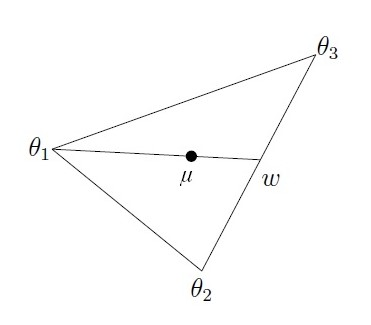
\includegraphics[scale=0.7]{triangle}
\caption{Ilustracija postopka določanja izotropnega vektorja za točko v konveksni ogrinjači treh točk iz $W(A)$.}
\label{fig:triangle}
\end{figure}
Naj bo $\varepsilon >0$ toleranca (npr. $\varepsilon=10^{-16}\norm{A}$ za dvojno natančnost). 
\paragraph{Algoritem:}
\begin{enumerate}[1.]
\item Poiščemo zunanjo aproksimacijo $W(A)$ (je pravokotnik, katerega stranice so vzporedne z realno in imaginarno osjo), tako da zračunamo najbolj levo in najbolj desno lastno vrednost $H_\theta =(e^{i\theta}A+e^{-i\theta}A^\ast)/2$ za $\theta =0, \pi/2$. %S tem dobimo zunanjo aproksimacijo zaloge vrednosti, ki seka $\partial W(A)$ v robnih točkah. %RAZLAGA Zunanja aproksimacija bo pravokotnik, katerega stranice so vzporedne z realno in imaginarno osjo. 
Če $\mu$ ni v zunanji aproksimaciji, potem $\mu \not \in W(A)$ in ustavimo algoritem, drugače nadaljujemo.
\item Če je višina ali širina zunanje aproksimacije manj kot $\varepsilon$, potem je $W(A)$ približno hermitska ali poševno-hermitska (ali kompleksen premik katere od teh) in je numerični zaklad približno točka. V obeh primerih ugotovimo ali je $\mu \in W(A)$. Če je, poiščemo pripadajoč izotropni vektor. 
\item Če $\mu \not \in W(A)$, nadaljujemo s konstrukcijo notranje aproksimacije $W(A)$ (je štirikotnik z oglišči v robnih točkah $\partial W(A)$) z uporabo lastnih vektorjev najbolj leve in desne lastne vrednosti $H_{\theta}$.% RAZLAGA Notranja aproksimacija bo štirikotnik z oglišči v robnih točkah $\partial W(A)$.
\item  Če $\mu$ leži v notranji aproksimaciji, lahko poiščemo izotropni vektor, ki generira $\mu$. Uporabimo postopek, ki je bil opisan v začetku tega razdelka. %OPISS
Če $\mu$ ne leži v notranji aproksimaciji, določimo katera stranica notranje aproksimacije mu leži najbližje.
\item  Izračunamo $\hat{\mu}$, ki je najbližja točka do $\mu$, ki leži na notranji aproksimaciji. Če je $\abs{\hat{\mu}-\mu}<\varepsilon$, izračunamo izotropni vektor za $\hat{\mu}$ in ga sprejmemo kot izotropni vektor za $\mu$ ter ustavimo algoritem.
\item Posodobimo notranjo in zunanjo aproksimacijo z izračunom največje lastne vrednosti in pripadajočega lastnega vektorja $H_{\theta}$, kjer je smer $\theta$ pravokotna na stranico notranje aproksimacije, ki je najbližja $\mu$. Če ne dobimo nove robne točke, ki se ni dotikala notranje aproksimacije, potem $\mu \not \in W(A)$. 
\item Ponovno preverimo, če je $\mu$  v novi zunanji aproksimaciji. Če je, se vrnemo na 4. korak, drugače $\mu \not \in W(A)$. 
\end{enumerate}
\begin{opomba}
Korake 4.-7. ponavljamo, dokler ni notranja aproksimacija $\varepsilon$ blizu $\mu$ ali dokler zunanja aproksimacija ne vsebuje $\mu$. Carden trdi, da se v večini primerov postopek konča v koraku 4. po le nekaj ponavljanjih.(\cite{carden})
\end{opomba}}
%Zunanja aproksimacija numeričnega zaklada, ki seka $\partial W(A)$ v robnih točkah, bo pravokotnik, katerega stranice so vzporedne z realno in imaginarno osjo,  notranja aproksimacija pa štirikotnik z oglišči v robnih točkah $\partial W(A)$.
%VKLJUČIM POPRAVEK?
%Ta algoritem ne izkoristi dejstva, da je numerični zaklad $2\times2$ matrike elipsa. Ta lastnost nakazuje, da z točkami in pripadajočimi izotropnimi vektorji za notranjo aproksimacijo, lahko natančno določimo izotropne vektorje za točke zunaj notranje aproksimacije. Tako lahko korak 5. popravimo:
%\begin{enumerate}[5.]
%\item Preverimo, če $\mu$ leži na elipsi
%\end{enumerate}
 %Definiraj genarirajoč vektor in ritzove vrednosti
 %%%%%%%%%%%%%%%%%%%%%%%%%%%%%%%%%%%%%%%%%%%%%%%%%%%%%%%%%%%%%%%%%%%%%%%%%%%%%%%%%%%%%%%%%%%%%%%%%%%%%%%%%%%%%%%%%%
\subsubsection{Chorianopoulos, Psarrakos in Uhlig.}
V tem razdelku opišemo algoritem Chorianopoulosa, Psarrakosa in Uhliga (označimo s CPU) za inverzen problem numeričnega zaklada.
Algoritem je hitrejši in daje natančne numerične rezultate tam, kjer se zgornja algoritma mnogokrat ustavita. Tak primer je ko $\mu$ ($\in W(A)$ ali $\not\in W(A)$) leži zelo blizu roba numeričnega zaklada $\partial W(A)$ (\cite{trije}). Ta algoritem uporabi za iskanje izotropnih vektorjev le nekaj najbolj osnovnih lastnosti numeričnega zaklada poleg konveksnosti, kot sta (4) in (5).\\
\paragraph{Algoritem:}
\begin{enumerate}[1.]
\item Izračunamo do 4 robne točke numeričnega zaklada $p_i$ in njihove izotropne vektorje $b_i$ za $i=1,2,3,4$, tako da izračunamo ekstremne lastne vrednosti, ki pripadajo enotskim lastnim vektorjem $x_i$ %a je to isti x oz. b?
matrike $H$ in $K$.
\item Nastavimo $p_i =b^\ast _i Ab_i$. Dobimo 4 točke $p_i$, ki označujejo ekstremne vrednosti $W(A)$, tj. najmanjši in največji horizontalni in vetikalni razteg. Označimo jih z $rM$ in $rm$ za maksimalen in minimalen horizontalni razteg $W(A)$ in z $iM$ in $im$ za maksimalen in minimalen vertikalen razteg $W(A)$. Če je $|p_i|<10^{-13}$ za $i=1,2,3,4$, potem je naš izotropni vektor kar pripadajoč enotski vektor.
\item Če med računanjem lastnih vektorjev in lastnih vrednosti ugotovimo, da je ena od matrik $H$ in $K$ definitna, t.j. da imajo njene lastne vrednosti vse enak predznak, potem vemo, da $\mu \not\in W(A),$ in algoritem ustavimo.
\item Narišemo elipse, ki so preslikave velikega kroga kompleksne sfere $\C^n$, ki gredo skozi vse možne pare točk $rm, rM, im$ in $iM$, ki imajo nasprotno predznačene imaginarne dele. Nato izračunamo presečišča vsake dobljene elipse z realno osjo.%Poiščemo presečišča realne osi z elipsami, ki so preslikave velikega kroga kompleksne sfere $\C^n$, %ko $x\mapsto x^\ast Ax$, ki grejo skozi vse možne pare izračunanih točk $p_i=x^\ast Ax$, $p_j=y^\ast  Ay$, tj. pari, ki imajo nasprotno predznačene imaginarne dele.
\item Če so izračunana presečišča na obeh straneh 0, potem izračunamo izotropni vektor z lemo \ref{komp}.
\item Če presečišča niso na obeh straneh 0, potem moramo rešiti kvadratno enačbo 
\begin{align}\label{eq:en3}
(tx +(1-t)y)^\ast A(tx+(1-t)y) & =(x^\ast Ax+y^\ast Ay -(x^\ast Ay +y^\ast Ax))t^2 \\
&+(-2y^\ast Ay +(x^\ast Ay+y^\ast Ax))t +y^\ast Ay.\nonumber
\end{align}
Njene ničle določijo koordinatne osi $W(A)$ točk na elipsah skozi točke $x^\ast Ax$, $y^\ast Ay\in \partial W(A)$ %?????
in so generirane s točkami v $\C^n$ na velikem krogu skozi $x$ in $y$. 
\item To je kvadratna enačba s kompleksnimi števili. Nas zanimajo samo rešitve, ki imajo imaginaren del enak 0, saj želimo uporabiti lemo \ref{komp}.
Če imaginarni del enačbe \eqref{eq:en3} enačimo z 0, dobimo naslednjo polinomsko enačbo z realnimi koeficienti:
\begin{equation}
t^2+gt+\frac{p}{f}=0 \label{eq:en4}
\end{equation}
za $q=\Im(x^\ast Ax)$, $p=\Im(y^\ast Ay)$ in $r=\Im(x^\ast  Ay + y^\ast Ax)$. Označimo $f=p+q-r$ in $g=(r-2p)/f$.
\item  Enačba \eqref{eq:en4} ima realni rešitvi $t_i$, $i=1,2$, ki vrneta generirajoča vektorja $b_i=t_ix+(1-t_i)y$ ($i=1,2$) za realni točki. Z normalizacijo dobimo izotropne vektorje. %SLIKA
\item Če nobena od možnih elips ne seka realno os na vsaki strani 0, potem preverimo, če to stori njihova skupna množica in ponovimo isti postopek.
\item Če niti skupna množica ne gre, potem izračunamo še več lastnih vrednosti in lastnih vektorjev za $A(\theta)=\cos(\theta)H+\sin(\theta)K$ za kote $\theta \not =0,\pi/2$ in delamo bisekcijo med točkami $rm$, $rM$, $im$, $iM$.
\item Končamo, ko najdemo definitno matriko $A(\theta)$ ali elipso, ki seka realno os na obeh straneh 0, nakar lahko uporabimo lemo \ref{komp}.
\end{enumerate}
%%%%%%%%%%%%%%%%%%%%%%%%%%%%%%%%%%%%%%%%%%%%%%%%%%%%%%%%%%%%%%%%%%%%
\section{Numerična analiza}
V tem poglavju bomo na kratko opisali naš algoritem, ki je povzet po algoritmu \ref{Meurant 2} iz \cite{meurant}, vendar pa ni identičen, in ga primerjali z algoritmoma Cardna iz \cite{carden_alg} in CPU iz \cite{trije_alg} na različnih primerih problema iskanja izotropnih vektorjev. 
%%%%%%%%%%%%%%%%%%%%%%%%%%%%%%%%%%%%%%%%%%%%%%%%%%%%%%%%%%%%%%%%%%%%%%%%%
\subsection{Opis algoritma}
Najprej na kratko opišimo kako naš algoritem, najden v poglavju 6, deluje. \\
Prva stvar, ki jo algoritem naredi, je da problem \eqref{eq:splosno} preobrne v začetni problem \eqref{eq:zac}. Nato preveri, če je matrika $A$ realna in če je, pokliče funkcijo \verb+izotropniMeurantR+, ki vrne 2 izotropna vektorja, izračunana kot v poglavju \ref{Realne matrike}. Nadalje algoritem uporabi isti postopek kot je opisan v \ref{Meurant 2}, tako da poskusi rešiti problem z lastnimi vektorji matrike $K$, če to ne deluje poskusi z lastnimi vektorji matrike $H$ in na koncu še s kombinacijo lastnih vektorjev matrike $K$ in $H$. V članku \cite{meurant} ni napisano koliko lastnih vektorjev je potrebno oz. se jih splača izračunati, zato smo to določili sami in sicer naš algoritem računa z lastnimi vektorji, ki pripadajo 3 največjim in 3 najmanjšim lastnim vrednostim. Edina razlika med našim algoritmom in algoritmom iz \ref{Meurant 2} nastane zaradi premalo informacij iz članka \cite{meurant} o tem kako najti vektorja $b_1$ in $b_2$, da lahko uporabimo lemo \ref{komp}. Naš algoritem najde $b_1$ in $b_2$ tako kot je opisano v koraku 4. in 5. algoritma, ko kombiniramo lastne vektorje matrike $K$ in $H$, kar naredi funckija \verb+xtheta+. Torej upoštevamo vektorje $X_\theta =\cos(\theta)x+\sin(\theta)y$, $0\le\theta\le\pi$, kjer $X_\theta ^\ast AX_\theta$ opiše elipso znotraj numeričnega zaklada. Za dan par $(x,y)$ iščemo presečišča elipse $X_\theta ^\ast AX_\theta$ z realno osjo, kjer sta $x$ in $y$ lastna vektorja matrike $K$ ali matrike $H$ in ti presečišči vzamemo kot kandidata za $b_1$ in $b_2$. Vendar naš algoritem ta korak še izboljša, saj maksimizira elipso $X_\theta ^\ast AX_\theta$, tako da $X_\theta$ definiramo kot $$X_\theta (\varphi) =\cos(\theta)x e^{\varphi \imath}+\sin(\theta)y,$$ kjer je $$\varphi = \frac{1}{2\imath} \text{ln}(x^\ast Ay (y^\ast Ax)^{-1}).$$ Če maksimiziramo elipso je večja verjetnost, da bo vsebovala izhodišče in s tem je večja verjetnost, da najdemo rešitev v manj korakih. Če najdemo primerna $b_1$ in $b_2$ da lahko uporabimo lemo \ref{komp}, ki je definirana s funkcijo \verb+lema31+, smo končali.
%%%%%%%%%%%%%%%%%%%%%%%%%%%%%%%%%%%%%%%%%%%%%%%%%%%%%%%%%%%%%%%%%%%%%%%
\subsection{Primerjava}
O\-zna\-či\-mo algoritme z \verb+AlgM+, \verb+AlgC+ in \verb+AlgCPU+. Numerične zaklade bomo narisali s funkcijo iz \cite{fovals}, ki nariše tudi lastne vrednosti matrike $A$ s križci.
%%%%%%%%%%%%%%%%%%%%%%%%%%%%%%%%%%%%%%%%%%%%%%%%%%%%%%%%%%%%%%%%%%
\subsubsection{A in $\mu$ realna}

Za prvi primer vzamimo naključno generirano $10\times 10$ realno matriko $A$ in $\mu = 1,0419$, ki je znotraj numeričnega zaklada, Slika \ref{fig:p1}.
$$\verb+A = randn(10)+$$

\begin{figure}[!h]
\centering
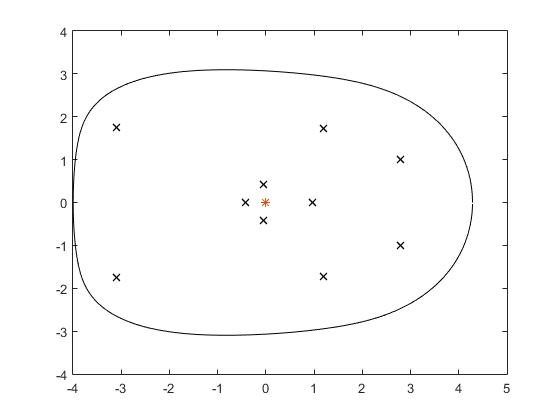
\includegraphics[scale=0.4]{RR1.jpg}
\caption{Numerični zaklad premaknjene matrike A in z rdečo $\ast$ označeno izhodišče.}
\label{fig:p1}
\end{figure}

\begin{table}[H]
\begin{tabular}{|l|l|c|r|}
\hline
Algoritem & Čas & Koraki & Napaka\\
\hline
\hline
\verb+AlgM+ & & & \\
\hline
\verb+AlgC+ & & & \\
\hline
\verb+AlgCPU+ & & & \\
\hline
\end{tabular}
\caption{A realna, $\mu = 1,0419$ in obstaja rešitev}
\label{t1}
\end{table}
Za drugi primer vzamimo $\mu =0$ in matriko
\begin{equation*}
A=\begin{bmatrix}
2 &-1&0\\
-1&2&-1\\
0&-1&2
\end{bmatrix}.
\end{equation*}
Matrika $A$ je definitna, zato algoritem ne najde rešitve.

\begin{table}[H]
\begin{tabular}{|l|l|c|r|}
\hline
Algoritem & Čas & Koraki & Napaka\\
\hline
\hline
\verb+AlgM+ & & & \\
\hline
\verb+AlgC+ & & & \\
\hline
\verb+AlgCPU+ & & & \\
\hline
\end{tabular}
\caption{A realna in ne obstaja rešitev.}
\label{t2}
\end{table}
%%%%%%%%%%%%%%%%%%%%%%%%%%%%%%%%%%%%%%%%%%%%%%%%%%%%%%%%%%%%%%%%%%%%%%%%
\subsubsection{A realna, $\mu$ kompleksen}


Naj bo $A$ naključno generirana realna $10\times 10$ matrika in $\mu = -1,4575 + 0,1514 \imath$ kompleksno število iz numeričnega zaklada, Slika \ref{fig:p31}.

\begin{figure}[H]
\begin{subfigure}[t]{0.5\textwidth}
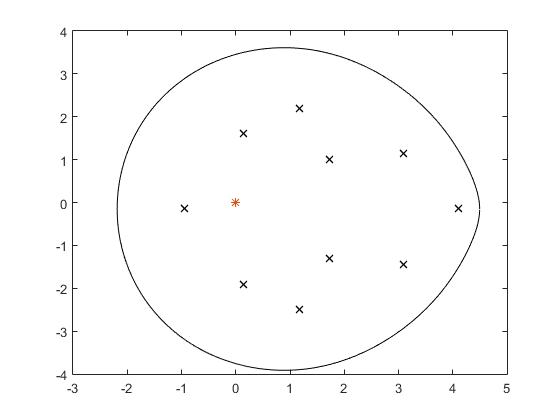
\includegraphics[width=0.9\linewidth]{RC1.jpg}
\caption{Z rdečo $\ast$ označimo izhodišče.}
\label{fig:p31}
\end{subfigure}%
\hfill
\begin{subfigure}[t]{0.5\textwidth}
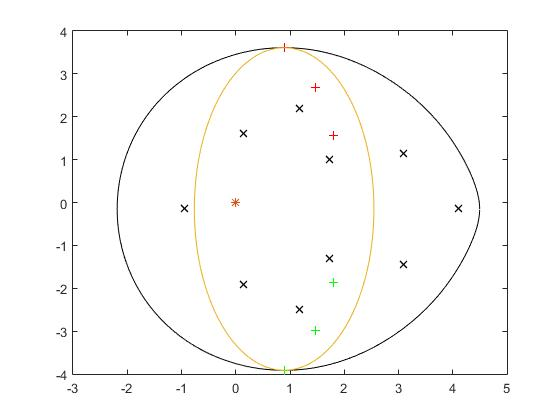
\includegraphics[width=0.9\linewidth]{RC1e.jpg}
\caption{Rdeči \verb~+~ so največji lastni vektorji, zeleni pa najmanjši lastni vektorji matrike K.}
\end{subfigure}
\caption{Numerični zaklad premaknjene matrike A in kako grafično najdemo rešitev v 1 koraku.}

\end{figure}

\begin{table}[H]
\begin{tabular}{|l|l|c|r|}
\hline
Algoritem & Čas & Koraki & Napaka\\
\hline
\hline
\verb+AlgM+ & & & \\
\hline
\verb+AlgC+ & & & \\
\hline
\verb+AlgCPU+ & & & \\
\hline
\end{tabular}
\caption{A realen, $\mu = -1,4575 + 0,1514 \imath$ in rešitev najdemo v 1 koraku.}
\label{t3}
\end{table}

Za drugi primer vzamemo realno naključno generirano $20\times 20$ matriko A in $\mu = 1 + \imath$, Slika \ref{fig:p41}.
\begin{figure}[H]
\begin{subfigure}[t]{0.5\textwidth}
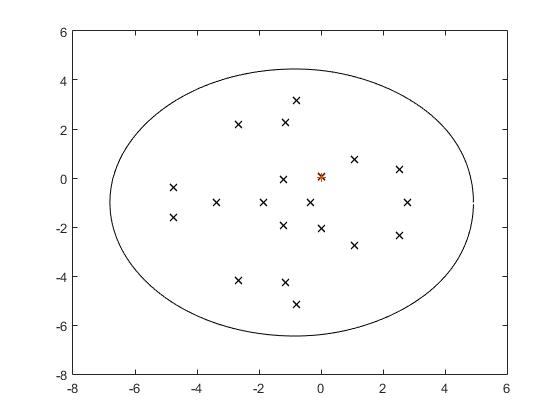
\includegraphics[width=0.9\linewidth]{RC2.jpg}
\caption{Z rdečo $\ast$ označimo izhodišče.}
\label{fig:p41}
\end{subfigure}%
\hfill
\begin{subfigure}[t]{0.5\textwidth}
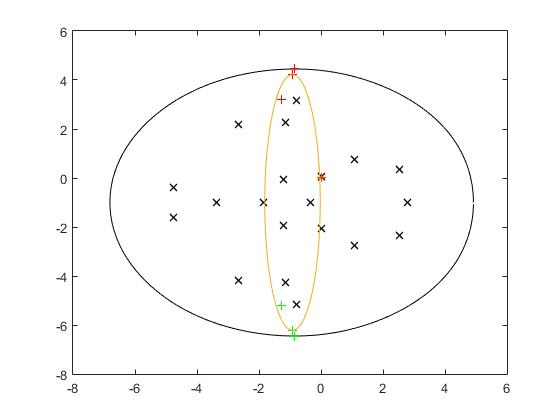
\includegraphics[width=0.9\linewidth]{RC2e1.jpg}
\caption{Rdeči \verb~+~ so največji lastni vektorji, zeleni pa najmanjši lastni vektorji matrike $K$\footnotemark. Z nobeno kombinacijo ne dobimo dovolj velike elipse, ki bi vsebovala izhodišče.}
\label{fig:p42}
\end{subfigure}
\hfill
\begin{subfigure}[t]{0.5\textwidth}
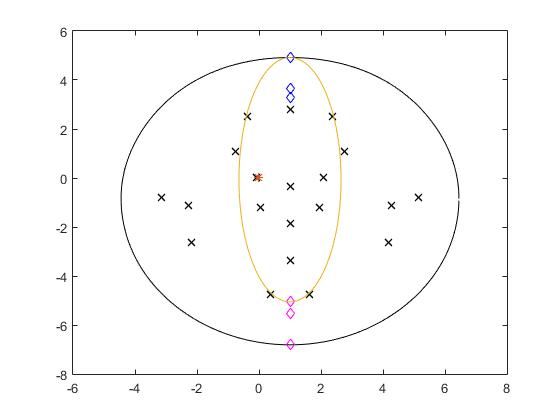
\includegraphics[width=0.9\linewidth]{RC2e2.jpg}
\caption{Modri $\diamond$ so največji lastni vektorji, roza pa najmanjši lastni vektorji matrike $H$\footnotemark[\value{footnote}]. Rišemo elipse za matriko $\imath A$.}
\label{fig:p43}
\end{subfigure}
\caption{Numerični zaklad premaknjene matrike $A$ in kako grafično najdemo rešitev v 2 korakih.}
\end{figure}

\begin{table}[H]
\begin{tabular}{|l|l|c|r|}
\hline
Algoritem & Čas & Koraki & Napaka\\
\hline
\hline
\verb+AlgM+ & & & \\
\hline
\verb+AlgC+ & & & \\
\hline
\verb+AlgCPU+ & & & \\
\hline
\end{tabular}
\caption{A realen, $\mu = 1 + \imath$ in rešitev najdemo v 2 korakih.}
\label{t4}
\end{table}

Za tretji primer vzamemo realno naključno generirano $20\times 20$ matriko A in $\mu = 2 + 2\imath$, Slika \ref{fig:p51}.
\begin{figure}[H]
\begin{subfigure}[t]{0.45\textwidth}
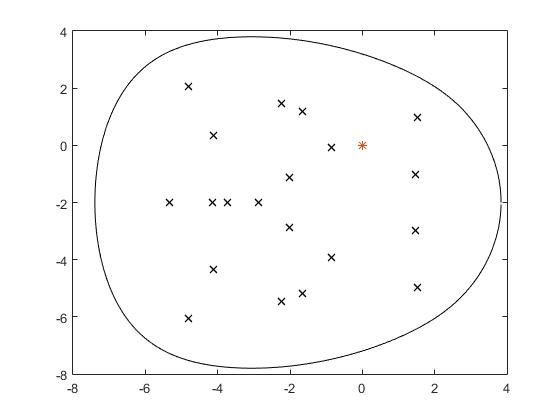
\includegraphics[width=0.9\linewidth,height=5cm]{RC3.jpg}
\caption{Z rdečo $\ast$ označimo izhodišče.}
\label{fig:p51}
\end{subfigure}%
\hfill
\begin{subfigure}[t]{0.45\textwidth}
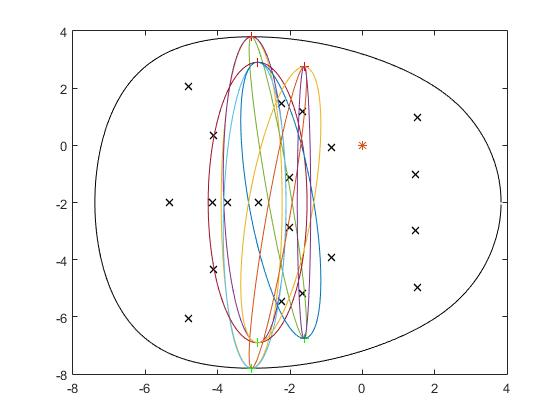
\includegraphics[width=0.9\linewidth,height=5cm]{RC3e1.jpg}
\caption{Rdeči \verb~+~ so največji lastni vektorji, zeleni pa najmanjši lastni vektorji matrike $K$\footnotemark[\value{footnote}]. Z nobeno kombinacijo ne dobimo dovolj velike elipse, ki bi vsebovala izhodišče.}
\label{fig:p52}
\end{subfigure}
\begin{subfigure}[t]{0.45\textwidth}
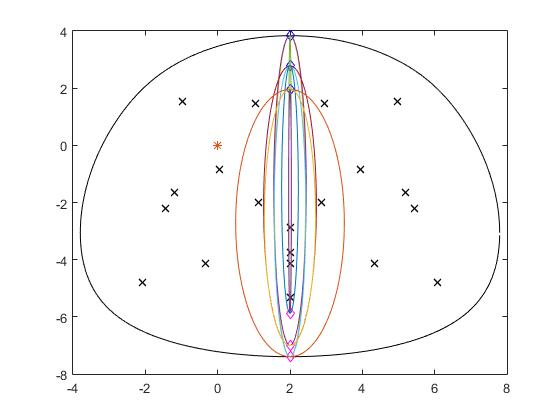
\includegraphics[width=0.9\linewidth,height=5cm]{RC3e2.jpg}
\caption{Modri $\diamond$ so največji lastni vektorji, roza pa najmanjši lastni vektorji matrike $H$\footnotemark[\value{footnote}]. Rišemo elipse za matriko $\imath A$. Z nobeno kombinacijo ne dobimo dovolj velike elipse, ki bi vsebovala izhodišče.}
\label{fig:p53}
\end{subfigure}%
\hfill
\begin{subfigure}[t]{0.45\textwidth}
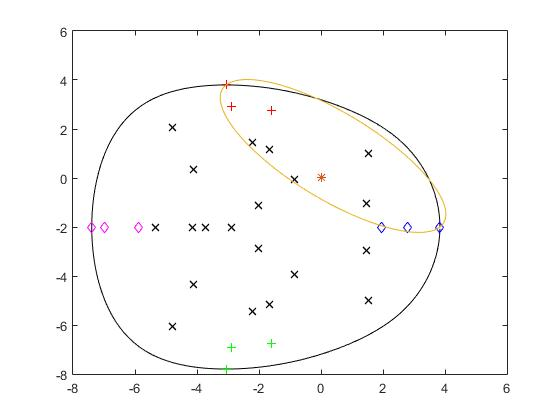
\includegraphics[width=0.9\linewidth,height=5cm]{RC3e3.jpg}
\caption{Gledamo vse kombinacije lastnih vektorjev $K$ in $H$ na matriki $A$\footnotemark[\value{footnote}].}
\label{fig:p53}
\end{subfigure}
\caption{Numerični zaklad premaknjene matrike $A$ in kako grafično najdemo rešitev v 3 korakih.}
\end{figure}

\begin{table}[H]
\begin{tabular}{|l|l|c|r|}
\hline
Algoritem & Čas & Koraki & Napaka\\
\hline
\hline
\verb+AlgM+ & & & \\
\hline
\verb+AlgC+ & & & \\
\hline
\verb+AlgCPU+ & & & \\
\hline
\end{tabular}
\caption{A realen, $\mu = 2 + 2\imath$ in rešitev najdemo v 3 korakih.}
\label{t5}
\end{table}

Poglejmo še en primer, kjer algoritem ne deluje za realno naključno generirano $50\times 50$ matriko A in $\mu = -8+4\imath$, ki je na robu numeričnega zaklada, Slika \ref{fig:p61}.
\begin{figure}[H]
\begin{subfigure}[t]{0.45\textwidth}
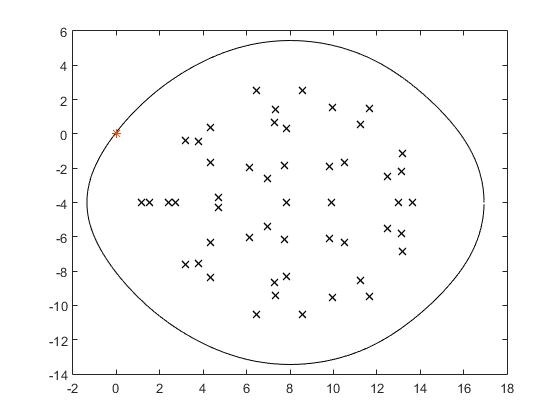
\includegraphics[width=0.9\linewidth,height=5cm]{RC4.jpg}
\caption{Z rdečo $\ast$ označimo izhodišče.}
\label{fig:p61}
\end{subfigure}%
\hfill
\begin{subfigure}[t]{0.45\textwidth}
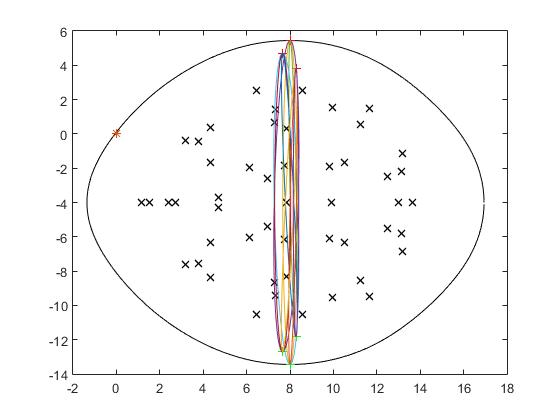
\includegraphics[width=0.9\linewidth,height=5cm]{RC4e1.jpg}
\caption{Rdeči \verb~+~ so največji lastni vektorji, zeleni pa najmanjši lastni vektorji matrike $K$\footnotemark[\value{footnote}]. Z nobeno kombinacijo ne dobimo dovolj velike elipse, ki bi vsebovala izhodišče.}
\label{fig:p62}
\end{subfigure}
\begin{subfigure}[t]{0.45\textwidth}
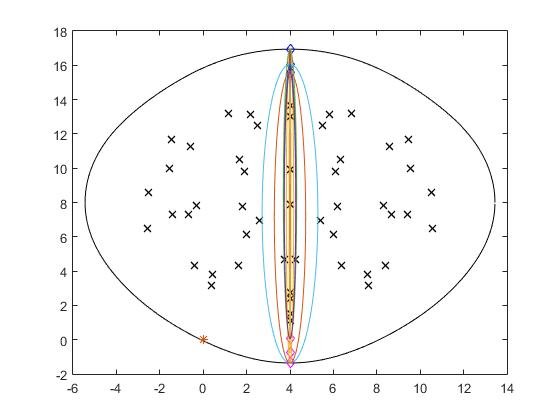
\includegraphics[width=0.9\linewidth,height=5cm]{RC4e2.jpg}
\caption{Modri $\diamond$ so največji lastni vektorji, roza pa najmanjši lastni vektorji matrike $H$\footnotemark[\value{footnote}]. Rišemo elipse za matriko $\imath A$. Z nobeno kombinacijo ne dobimo dovolj velike elipse, ki bi vsebovala izhodišče.}
\label{fig:p63}
\end{subfigure}%
\hfill
\begin{subfigure}[t]{0.45\textwidth}
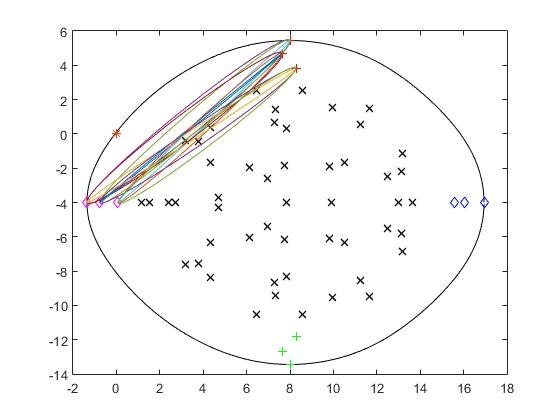
\includegraphics[width=0.9\linewidth,height=5cm]{RC4e3.jpg}
\caption{Gledamo vse kombinacije lastnih vektorjev $K$ in $H$ na matriki $A$\footnotemark[\value{footnote}]. Narisane so le tiste elipse, ki imajo možnost vsebovat izhodišče.}
\label{fig:p63}
\end{subfigure}
\caption{Numerični zaklad premaknjene matrike $A$ in kako grafično ne najdemo rešitve.}
\end{figure}

\begin{table}[H]
\begin{tabular}{|l|l|c|r|}
\hline
Algoritem & Čas & Koraki & Napaka\\
\hline
\hline
\verb+AlgM+ & & & \\
\hline
\verb+AlgC+ & & & \\
\hline
\verb+AlgCPU+ & & & \\
\hline
\end{tabular}
\caption{A realen, $\mu = -8+4\imath$ in naš algoritem ne najde rešitve.}
\label{t6}
\end{table}

%%%%%%%%%%%%%%%%%%%%%%%%%%%%%%%%%%%%%%%%%%%%%%%%%%%%%%%%%%%%%%%%%%%%%
\subsubsection{A in $\mu$ kompleksna}
V tem poglavju bomo za matriko $A$ vzeli matriko,  ki je uporabljena tudi v \cite{meurant} in \cite{trije}, velikosti $200\times 200$, ki se konstruira iz Fiedlerjeve $F$ in Molerjeve $M$ matrike. Potem je $B=F + \imath M$ in A (v Matlab kodi):
$$\verb~A=B+(-3+5i)*ones(200)-(200+500i)*eye(200)~$$

Za prvi primer vzamimo $\mu = 5000+10000\imath$, Slika \ref{fig:p7}.


\begin{table}[H]
\begin{tabular}{|l|l|c|r|}
\hline
Algoritem & Čas & Koraki & Napaka\\
\hline
\hline
\verb+AlgM+ & & & \\
\hline
\verb+AlgC+ & & & \\
\hline
\verb+AlgCPU+ & & & \\
\hline
\end{tabular}
\caption{A in $\mu$ kompleksna in algoritem najde rešitev v 1 koraku.}
\label{t7}
\end{table}

Za drugi primer vzamemo $\mu = 12000+10000\imath$, ki je bližje robu, Slika \ref{fig:p7}.

\begin{table}[H]
\begin{tabular}{|l|l|c|r|}
\hline
Algoritem & Čas & Koraki & Napaka\\
\hline
\hline
\verb+AlgM+ & & & \\
\hline
\verb+AlgC+ & & & \\
\hline
\verb+AlgCPU+ & & & \\
\hline
\end{tabular}
\caption{A kompleksna,$\mu = 5000+10000\imath$ in algoritem najde rešiev v 2 korakih.}
\label{t8}
\end{table}

Za tretji primer vzamemo $\mu = 12500+10000\imath$, ki je še bližje robu kot v prejšnjem primeru, Slika \ref{fig:p7}.


\begin{table}[H]
\begin{tabular}{|l|l|c|r|}
\hline
Algoritem & Čas & Koraki & Napaka\\
\hline
\hline
\verb+AlgM+ & & & \\
\hline
\verb+AlgC+ & & & \\
\hline
\verb+AlgCPU+ & & & \\
\hline
\end{tabular}
\caption{A kompleksna, $\mu = 12500+10000\imath$ in algoritem najde rešitev v 3 korakih.}
\label{t9}
\end{table}

Za zadnji primer vzamimo $\mu = 6000+16000\imath$, ki je blizu roba, ampak vseeno ni v numeričnem zakladu, Slika \ref{fig:p7}.


\begin{table}[H]
\begin{tabular}{|l|l|c|r|}
\hline
Algoritem & Čas & Koraki & Napaka\\
\hline
\hline
\verb+AlgM+ & & & \\
\hline
\verb+AlgC+ & & & \\
\hline
\verb+AlgCPU+ & & & \\
\hline
\end{tabular}
\caption{A kompleksna, $\mu = 6000+16000\imath$ in algoritem ne najde rešitve.}
\label{t10}
\end{table}

\begin{figure}[H]
\begin{subfigure}[t]{0.5\textwidth}
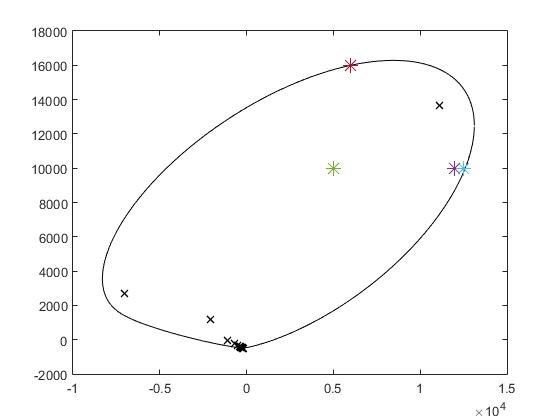
\includegraphics[width=0.9\linewidth]{CC.jpg}
\caption{Zelena $\ast = 5000+10000\imath$\\
Vijolična $\ast = 12000+10000\imath$\\
Modra $\ast = 12500+10000\imath$\\
Rdeča $\ast = 6000+16000\imath$\\}

\end{subfigure}%
\hfill
\begin{subfigure}[t]{0.5\textwidth}
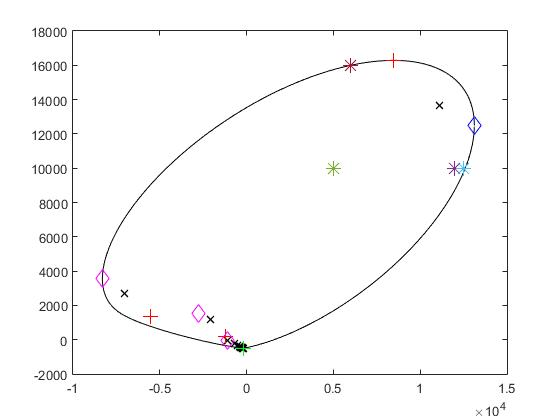
\includegraphics[width=0.9\linewidth]{CCC.jpg}
\caption{Rdeči \verb~+~ so največji lastni vektorji, zeleni pa najmanjši lastni vektorji matrike K. Modri $\diamond$ so največji lastni vektorji, roza pa najmanjši lastni vektorji matrike $H$.\footnotemark[\value{footnote}]}
\end{subfigure}
\caption{Numerični zaklad matrike A z dodanimi lastnimi vektorji\footnotemark[\value{footnote}] iz katere lahko za vsak primer hitro ugotovimo koliko korakov potrebujemo, da najdemo elipso, ki bo ali ne bo vsebovala $\mu$. }
\label{fig:p7}
\end{figure}

\footnotetext{Tukaj ne mislimo, da so v numeričnem zakladu narisani lastni vektorji, ampak točke, ki so izračunane s tem lastnim vektorjem. Npr. če je x naš lastni vektor, smo točko v numeričnem zakladu izračunali kot $x^\ast Ax$.}
%\subsection{Pričakovanjana}
%Za \verb+AlgM+ vemo, da če algoritem potrebuje le 1. korak, deluje hitrejše od ostalih dve algoritmov, saj porabi le eno računanje lastnih vektorjev in vrednosti. Če pa 1. korak ali 2. korak ne delujeta, je to potrata časa in druga dva algoritma delujeta hitreje.

\section{Zaključek}

\newpage
\section{Priloge}
\begin{verbatim}
function [b, napaka, korak] = izotropniMeurant(A, mu)
%ce je mozno, ta funkcija izracuna izotropne vektorje b, ki so
%resitev enacbe mu=b'Ab.
%Vhod: A...realna ali kompleksna matrika
%      mu ... kompleksno stevilo
%       
%
%Izhod:  b...izotropni vektor za mu
%        napaka ... norm(b'Ab-mu)
%        korak ... 0, če algoritem ne izračuna nobenih l. vekt.
%                  1, če algoritem izračuna le lastne vektorje K
%                  2, če algoritem izračna še lastne vektorje H
%                  3, če algoritem uporabi lastne vektorje K in H
warning off

if nargin ==1,
    mu=0;
    %tol = 1e-14;
end

[n, m] = size(A);
%preverimo, ce A kvadratna matrika
if n~=m,
    disp('Matrika A ni kvadratna!')
    return
end

%problem preobrnemo v b*(A-muI)b=0
A = A-mu*eye(n);

%A realna, algoritem za realne mtr.
if isreal(A)==1,
    [b, napaka, korak] = izotropniMeurantR(A);
    return
end

H=(A+A')/2;
K=(A-A')/(2*1i);
opts.disp = 0; 
opts.maxit = 1000; 
opts.tol = 10^-4;

napaka = Inf;
korak = 0;
b = 0;

[x, vred_k1] = eigs(K,3,'lr',opts); 

[y, vred_k2] = eigs(K,3,'sr',opts); 

korak = korak + 1;

X = [x,y];
LV = [diag(vred_k1);diag(vred_k2)];
for k=1: size(X,2)-1,
    for j = (k+1):size(X,2),
        if (LV(k,:)*LV(j,:) < 0),
            fi = (log(X(:,k)'*A*X(:,j)*inv(X(:,j)'*A*X(:,k))))/(2i); 
            %#ok<*MINV>
            [b1, b2] = xtheta(X(:,k)*exp(fi*1i), X(:,j), A);


            if sum(abs(b1)<ones(n,1)*1e-10)==0 && 
                sum(abs(b2)<ones(n,1)*1e-10)==0,
                b1 = b1/norm(b1);
                b2 = b2/norm(b2);

                if (abs(imag(b1'*A*b1))<1e-10) && 
                    (abs(imag(b2'*A*b2))<1e-10),
                    b = lema_31(b1,b2,A);
                    if sum(abs(b)<ones(n,1)*1e-10)==0,
                        napaka = abs(b'*A*b);
                        return
                    end
                end
            end
        end
    end

end


%ponovimo isti postopek za H in matriko iA
[xx, vred_h1] = eigs(H,3,'lr'); 

[yy, vred_h2] = eigs(H,3,'sr'); 

korak = korak + 1;

XX = [xx,yy];
LV1 = [diag(vred_h1);diag(vred_h2)];

for k=1: size(XX,2)-1,
    for j = (k+1): size(XX,2),
        if (LV1(k,:)*LV1(j,:)< 0),
          fi=(log(XX(:,k)'*A*XX(:,j)*inv(XX(:,j)'*A*XX(:,k))))/(2i);
            %#ok<*MINV>
            [b1, b2] = xtheta(XX(:,k)*exp(fi*1i), XX(:,j), 1i*A);

            if sum(abs(b1)<ones(n,1)*1e-10)==0 && 
                sum(abs(b2)<ones(n,1)*1e-10)==0,
                b1 = b1/norm(b1);
                b2 = b2/norm(b2);

                if (abs(imag(b1'*(1i*A)*b1))<1e-10) && 
                    (abs(imag(b2'*(1i*A)*b2))<1e-10),
                    b = lema_31(b1,b2,(1i*A));
                    if sum(abs(b)<ones(n,1)*1e-10)==0,
                        napaka = abs(b'*(1i*A)*b);
                        return
                    end
                end
            end
        end
    end
end

korak = korak +1;

for k=1:size(X,2),
    for j = 1: size(XX,2),
            fi=(log(X(:,k)'*A*XX(:,j)*inv(XX(:,j)'*A*X(:,k))))/(2i);
            %#ok<*MINV>
            [b1, b2] = xtheta(X(:,k)*exp(fi*1i), XX(:,j), A);

            if sum(abs(b1)<ones(n,1)*1e-10)==0 && 
                sum(abs(b2)<ones(n,1)*1e-10)==0,
                b1 = b1/norm(b1);
                b2 = b2/norm(b2);

                if (abs(imag(b1'*A*b1))<1e-10) &&
                    (abs(imag(b2'*A*b2))<1e-10),
                    b = lema_31(b1,b2,A);
                    if sum(abs(b)<ones(n,1)*1e-10)==0,
                        napaka = abs(b'*A*b);
                        return
                    end
                end
            end
    end
end        
disp('Algoritem ne najde resitve, uporabi algoritem CPU')

end

function [b, napaka, korak] = izotropniMeurantR(A)
%Resi problem iztotropnih vektorjev, če je matrika A realna in mi 
%realen oz. 0

%racunamo b'Hb=0
H=(A+A')/2;

opts.disp = 0; 
opts.maxit = 1000; 
opts.tol = 10^-4;

[x, vred_h1] = eigs(H,1,'la',opts); 

[y, vred_h2] = eigs(H,1,'sa',opts); 

if (vred_h1 * vred_h2) < 0,
    b1 = sqrt(vred_h1 / (vred_h1 + abs(vred_h2)))*y + 
    sqrt( abs(vred_h2) / (vred_h1 + abs(vred_h2)))*x;
    b2 = -sqrt(vred_h1 / (vred_h1 + abs(vred_h2)))*y + 
    sqrt( abs(vred_h2) / (vred_h1 + abs(vred_h2)))*x;
    b = [b1 ,b2];
    napaka = [abs(b1'*H*b1),abs(b2'*H*b2)];
    korak = 1;
else
    b = 0;
    napaka = Inf;
    korak = 0;
    disp('H je definitna')
end

function [b1,b2] = xtheta(x,y,A)

H=(A+ A')/2;
K=(A- A')/(2*1i);

alfa = imag(x'*H*x + 1i*x'*K*x);
beta = imag(y'*H*y + 1i*y'*K*y);
gama = imag(x'*H*y + y'*H*x + 1i*(x'*K*y + y'*K*x));

%resimo enacbo beta*t^2 + gama*t + alfa = 0
t1 = (-gama + sqrt(gama^2 -4*beta*alfa))/(2*beta);
t2 = (-gama - sqrt(gama^2 -4*beta*alfa))/(2*beta);

%preverimo, če sta resitvi realni
if (abs(imag(t1))<1e-10),
    theta1 = atan(real(t1));%t = tan(theta) 
    %(predpostavili smo, da cos(theta)~=0
    b1 = cos(theta1)*x + sin(theta1)*y;
else
    b1 = 0;
end

if (abs(imag(t2))<1e-10),
    theta2 = atan(real(t2));
    b2 = cos(theta2)*x + sin(theta2)*y;
else
    b2 = 0;
end
end

function [b] = lema_31(b1,b2,A)
%Vhod: enotska vektorja b1 in b2, za katera velja imag(bi'*A*bi)=0 za
%i=1,2, za dano matriko A
%Izhod: izotropni vektor b

a1 = real(b1'*A*b1);
a2 = real(b2'*A*b2);

if a1<0,
    if a2>0,
        alfa1 = a1;
        alfa2 = a2;
    else
        b=0;
        return
    end
elseif a1>0,
    if a2<0,
        alfa2 = a1;
        alfa1 = a2;
        [b2, b1] = deal(b1, b2);
    else
        b=0;
        return
    end
else
    b = 0;
    return
end
bb = @(t,th) exp(-1i*th)*b1 + t*b2;
al = @(th) exp(1i*th)*b1'*A*b2 + exp(-1i*th)*b2'*A*b1; 

th = angle(b2'*A*b1 - b1.'*conj(A)*conj(b2));
t1 = (-al(th) + sqrt(al(th)^2 -4*alfa1*alfa2))/(2*alfa2);

b = bb(t1,th)/norm(bb(t1,th));

end
\end{verbatim}



\vfill

% slovar
\section*{Slovar strokovnih izrazov}

\geslo{isotropic vector}{izotropni vektor}
\geslo{isotropic vector}{zrcalni zdrs ali zrcalni pomik -- tip ravninske evklidske izometrije, ki je kompozitum zrcaljenja in translacije vzdol"z iste premice}

\geslo{field of values/numerical range}{numerični zaklad}

\geslo{convex hull}{konveksna ogrinjača}

\geslo{partition}{\textbf{$\sim$ of a set} razdelitev mno"zice; \textbf{$\sim$ of a number} raz"clenitev "stevila}

% seznam uporabljene literature
% \cite{meurant} za referenco
\begin{thebibliography}{99}



\bibitem{carden}
R. Carden, \emph{A simple algorithm for the inverse field of values problem}, Inverse Probl. {\bf 25} (2009) 1--9

\bibitem{carden_alg}
R. Carden, \emph{\texttt{inversefov.m}}, verzija 6.~2.~2011, [ogled 5.~5.~2016], dostopno na \url{http://www.caam.rice.edu/tech_reports/2009/}.

\bibitem{trije}
C. Chorianopoulos, P. Psarrakos in F. Uhlig, \emph{A method for the inverse numerical range problem}, Electron. J. Linear Algebra {\bf 20} (2010) 198--206

\bibitem{lipkin}
N. Ciblak, H. Lipkin, \emph{Orthonormal isotropic vector bases}, In: Proceedings of DETC'98, 1998 ASME Design Engineering Technical Conferences (1998).

\bibitem{fovals}
W. Henao, \emph{\texttt{fovals.m}}, [ogled 29.~6.~2017], dostopno na \url{https://www.mathworks.com/matlabcentral/mlc-downloads/downloads/submissions/4679/versions/1/previews/fovals.m/index.html?access_key=}.

\bibitem{num}
Johnson, C. R., \emph{Numerical determination of the field of values of a general complex matrix}, SIAM J. Numer. Anal. {\bf 15} (1978) 595--602.

\bibitem{meurant}
G. Meurant, \emph{The computation of isotropic vectors}, Numer. Alg. {\bf 60} (2012) 193--204.

\bibitem{zaloga}
P. Psarrakos, M. Tsatsomeros, \emph{Numerical range: (in) a matrix nutshell} Math. Notes from Washington State University,  Vol 45, No. 2 (2002)

\bibitem{nr}
P. Psarrakos, \emph{\texttt{nr.m}}, [ogled 29.~6.~2017], dostopno na \url{http://www.math.wsu.edu/faculty/tsat/files/matlab/nr.m}.

\bibitem{trije_alg}
F. Uhlig, \emph{\texttt{invfovCPU.m}}, verzija 22.~3.~2011, [ogled 5.~5.~2016], dostopno na \url{http://www.auburn.edu/~uhligfd/m_files/invfovCPU.m}.

\end{thebibliography}

\end{document}


